\documentclass[a4paper]{article}
\usepackage[utf8]{inputenc}

\title{\textbf{SCALING OF MEAN EDGE LENGTH IN SYNTACTIC DEPENDENCY TREES}}
\author{ANKIT TEWARI }
\date{\today}

\usepackage{natbib}
\usepackage{graphicx}
\usepackage{caption}
\usepackage{tabularx}
\usepackage[a4paper]{geometry}
\usepackage{pdflscape}
\usepackage{rotating}
\usepackage{xspace}
\usepackage{float}
\usepackage{dcolumn}
\usepackage{tabu}
%\usepackage{subcaption}
\usepackage{tikz}
\usepackage{tkz-euclide}
\usetikzlibrary{calc,intersections,through,backgrounds}
%\usepackage{booktabs}
%\usepackage{multirow}
%\usepackage{multicol}
\usepackage{subfigure}


\begin{document}

\maketitle

\section{Introduction}
In this session, we attempted to fit a non-linear function to data using collections of syntactic dependency trees from different languages. In a syntactic dependency tree, the vertices are the words (tokens) of a sentence and links indicate syntactic dependencies between words [Ferrer-i-Cancho, 2013].
In this process, we created different models and tried to fit them on the data set of number of vertices (n) versus the mean length of the vertices of the tree (d)
	
\section[Data Pre-Processing]{Method}
\subsection{Processing of the original dataset}
There are two types of processed datasets that we have utilized for experimentation. Considering the original dataset for a particular language, the first kind of dataset was obtained on processing the original database in such a format that the first column of the processed dataset for each of the languages consists of the \textbf{number of nodes} for each syntactic dependency tree while the second column consists of \textbf{mean edge length} for the respective syntactic dependency tree. Each row of the processed dataset for a given language corresponds to a particular syntactic dependency tree and we compute the number of nodes of nodes and mean edge for each such row.\\
Also, while testing the data for \textit{\textbf{Homoscedasticty}}, we found that none of the languages were able to pass the \textit{\textbf{Breusch-Pagan test}}. This showed presence of heteroscedasticity.   

%\subsection{An overview of models under consideration}


\subsection{Model fitting}
We have considered the previously defined 9 different models to describe the relation between number of nodes and mean edge lengths for syntactic dependency trees for 30 different languages. In order to describe the abstract relation followed between these two metrics, we have employed the non-linear regression technique. 
\\
The non-linear regression can be invoked by means of the function nls(...). The function nls(...) requires a set of initial values in order to converge to the true solution and thus providing with parameters that are used to describe the non linear model. Under our present experimental conditions, we have tried to fit a linear model of log(number of nodes) versus log(mean edge length) and using the parameters obtained for drawing inferences about initial values for our non-linear regression.

\subsection{Model selection}
We have adopted a two phased approach based on double verification for model selection. Under this approach, we have employed the famous \textbf{\textit{Akaike Information Criterion (AIC)}} for model selection along with the values of \textbf{\textit{Residual Standard Errors (RSE)}} for each of the models under consideration described previously. 
\\
The first criteria that we had adopted was to examine the value of $\Delta$AIC and thereafter examine the value of RSE for the corresponding model. 


\section{Results}
There are some models that closely follow the logarithmic model while there are others that were following the exponential model. We have tried to exhibit the results in the form of plot of best models for each of the languages in the figures from \textbf{Figure 1} to \textbf{Figure 8}. 

 
The \textbf{table 1} provides a summary of properties of degree sequences. \textbf{Table 2} along with the \textbf{Table 3} describes results in the form of best parameters that are obtained on fitting the various models described previously on the dataset of syntactic dependency trees for 30 different languages. The list of all such languages under consideration is provided at the end of this report. \\
The \textbf{Table 4} provides a summary of the values of Akaike Information Criterion (AIC) obtained on fitting the 9 different models on the original data. In this series, we present the \textbf{Table 5} and \textbf{Table 6} which describe the results of $\Delta$AIC values and corresponding Residual Standard Errors.\\
Finally, we present the results of \textbf{Table 2 and Table 3} performed on aggregated datasets. we have describe the results in \textbf{Table 7 and table 8}. 
Similarily, the results of \textbf{Table 4, table 5 and Table 6} are summarized after being performed on the aggregated dataset. We have described the results in the form of a summary in \textbf{Table 9, Table 10 and Table 11}. 


\begin{figure*}[hbtp]
	\centering
	\subfigure[Arabic Language] {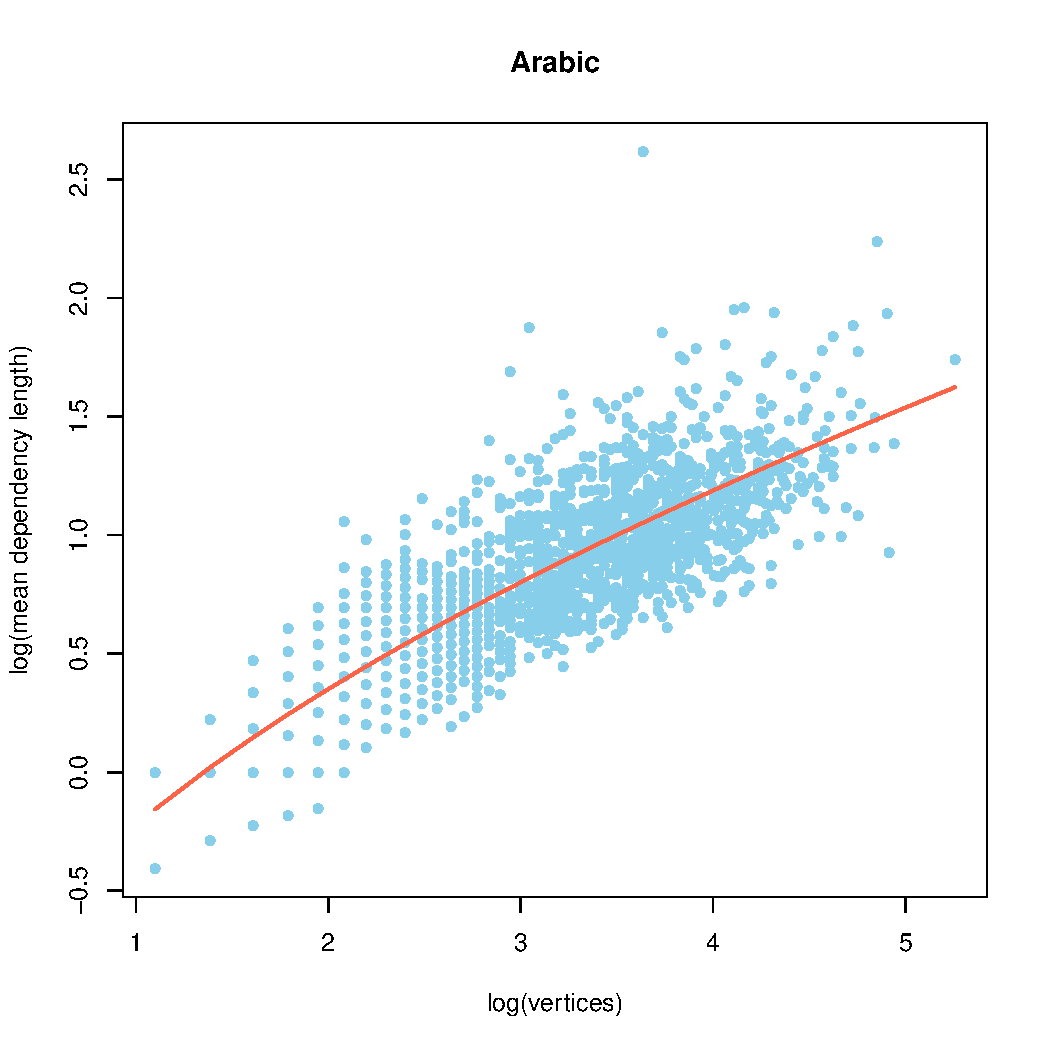
\includegraphics[scale=0.38]{Arabic}}\quad
	\subfigure[Basque Language]{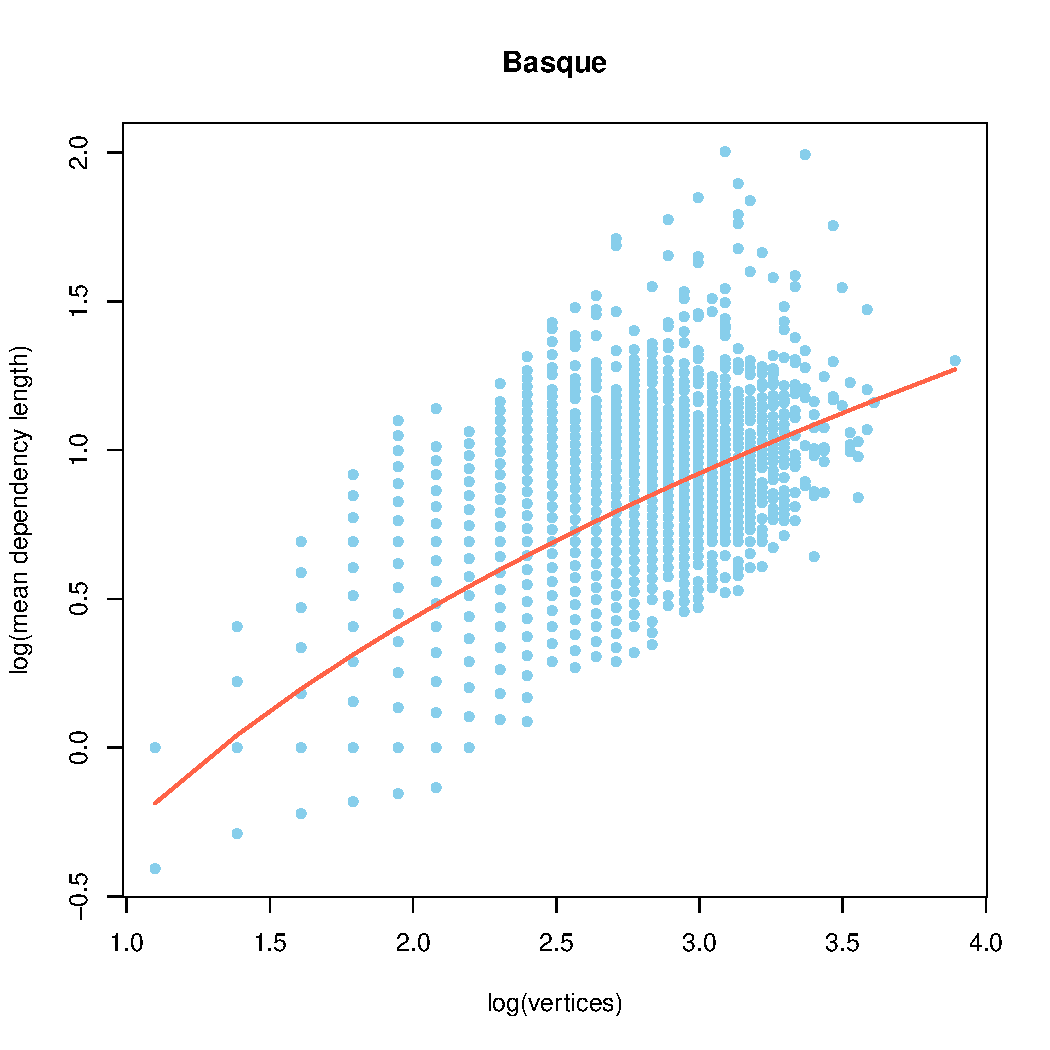
\includegraphics[scale=0.38]{Basque}}
	\caption{Plot of number of nodes versus mean edge length for different languages along with fitted curve following Model 2$+$}	
\end{figure*}

\begin{figure*}[hbtp]
	\centering
	\subfigure[Bulgarian Language]{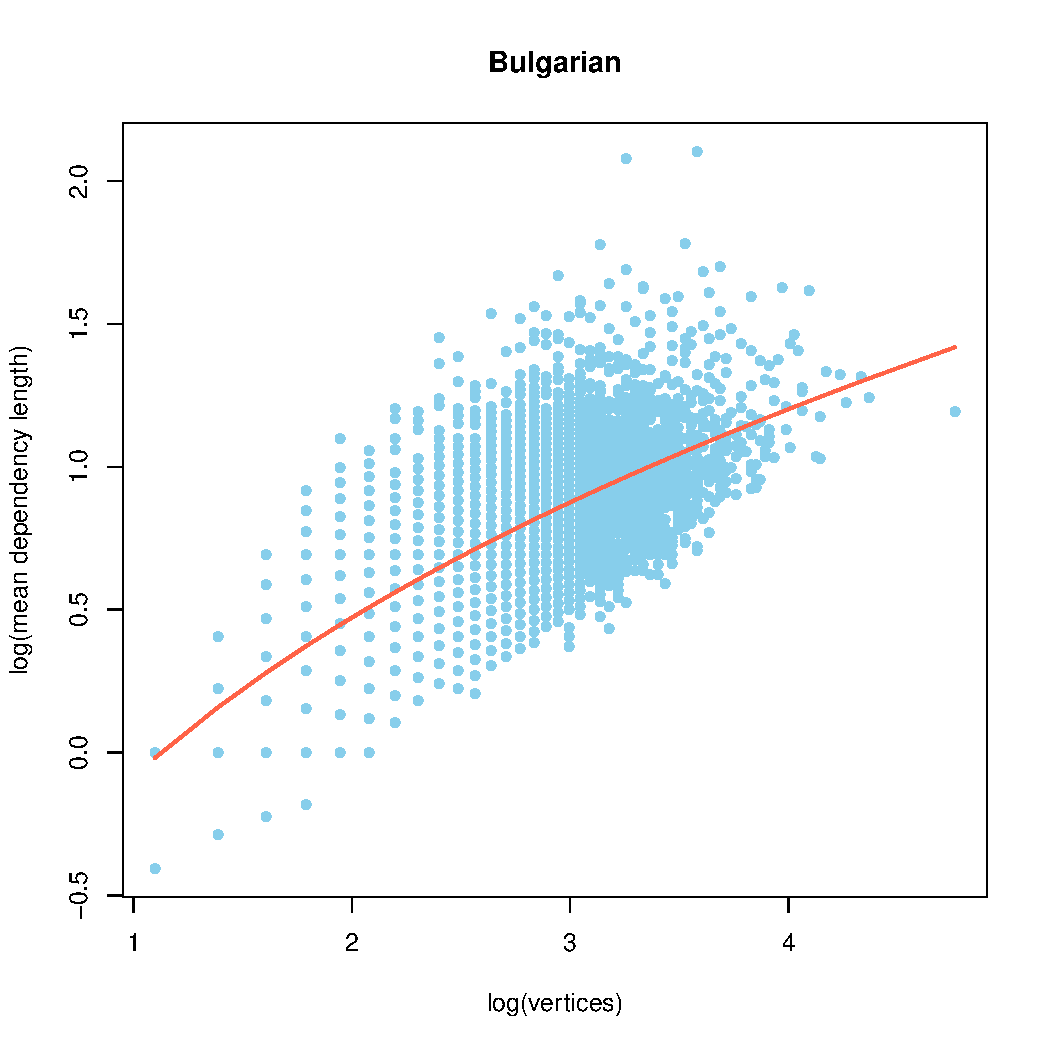
\includegraphics[scale=0.38]{Bulgarian}}\quad
	\subfigure[Catalan Language]{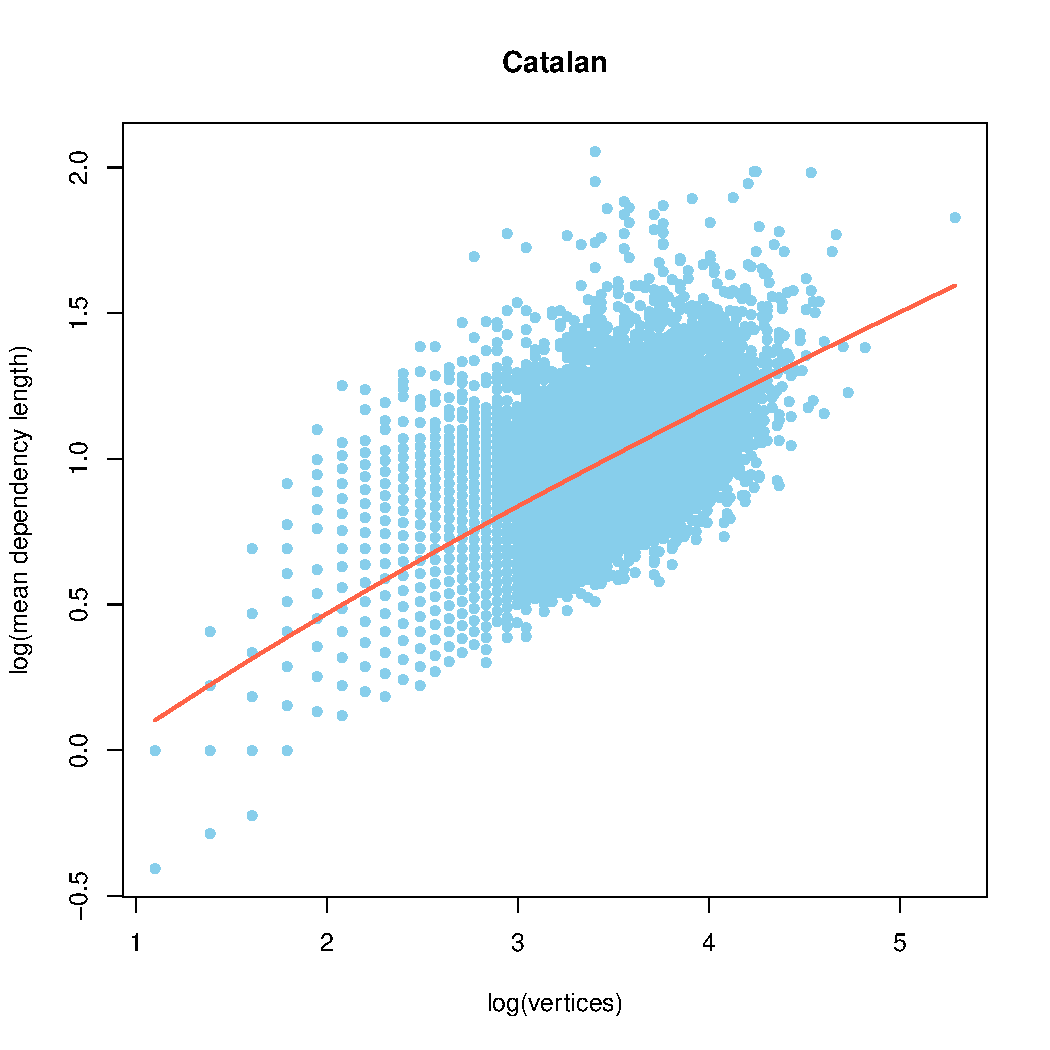
\includegraphics[scale=0.38]{Catalan}}
	\caption{Plot of number of nodes versus mean edge length for different languages along with fitted curve following Model 2$+$}
	
\end{figure*}

\begin{figure*}[hbtp]
	\centering
	\subfigure[Czech Language]{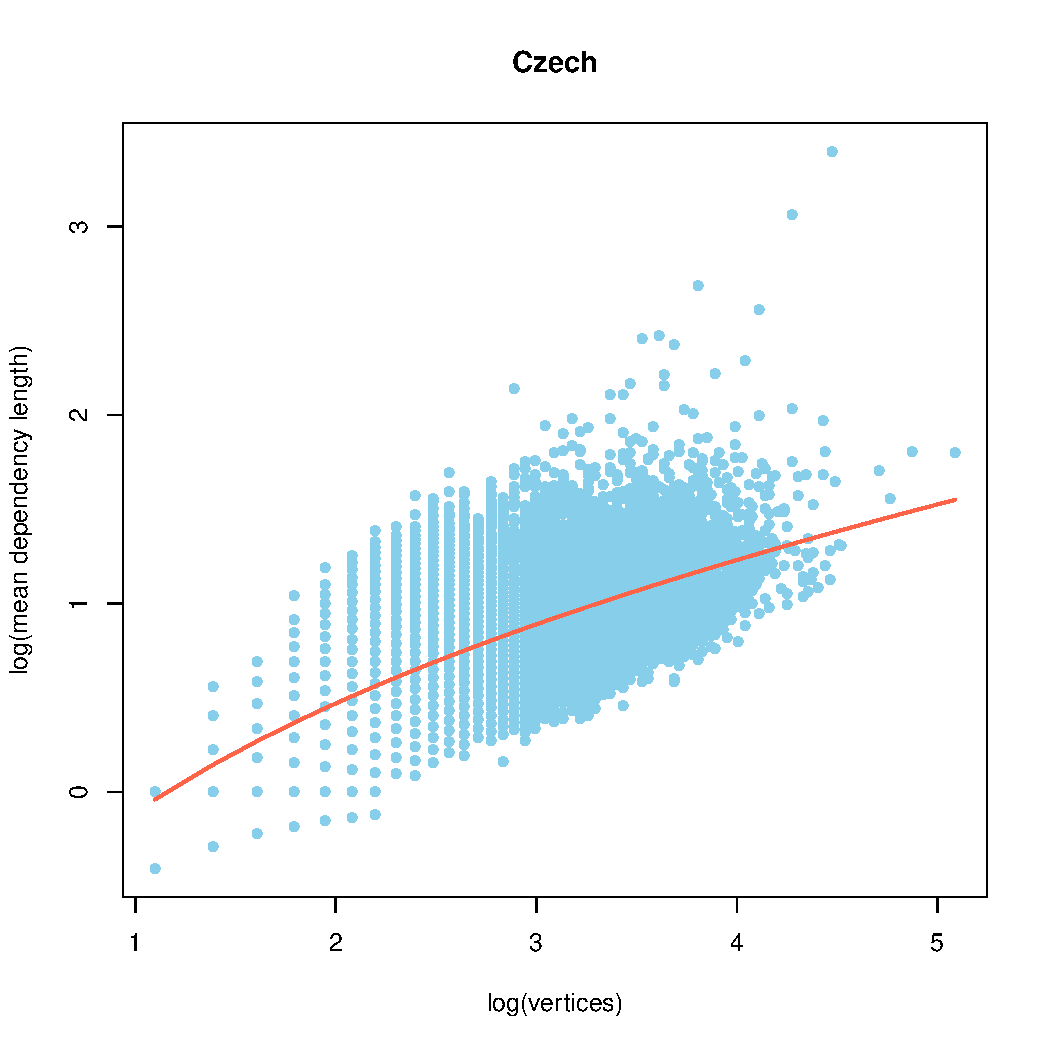
\includegraphics[scale=0.38]{Czech}}\quad
	\subfigure[English Language]{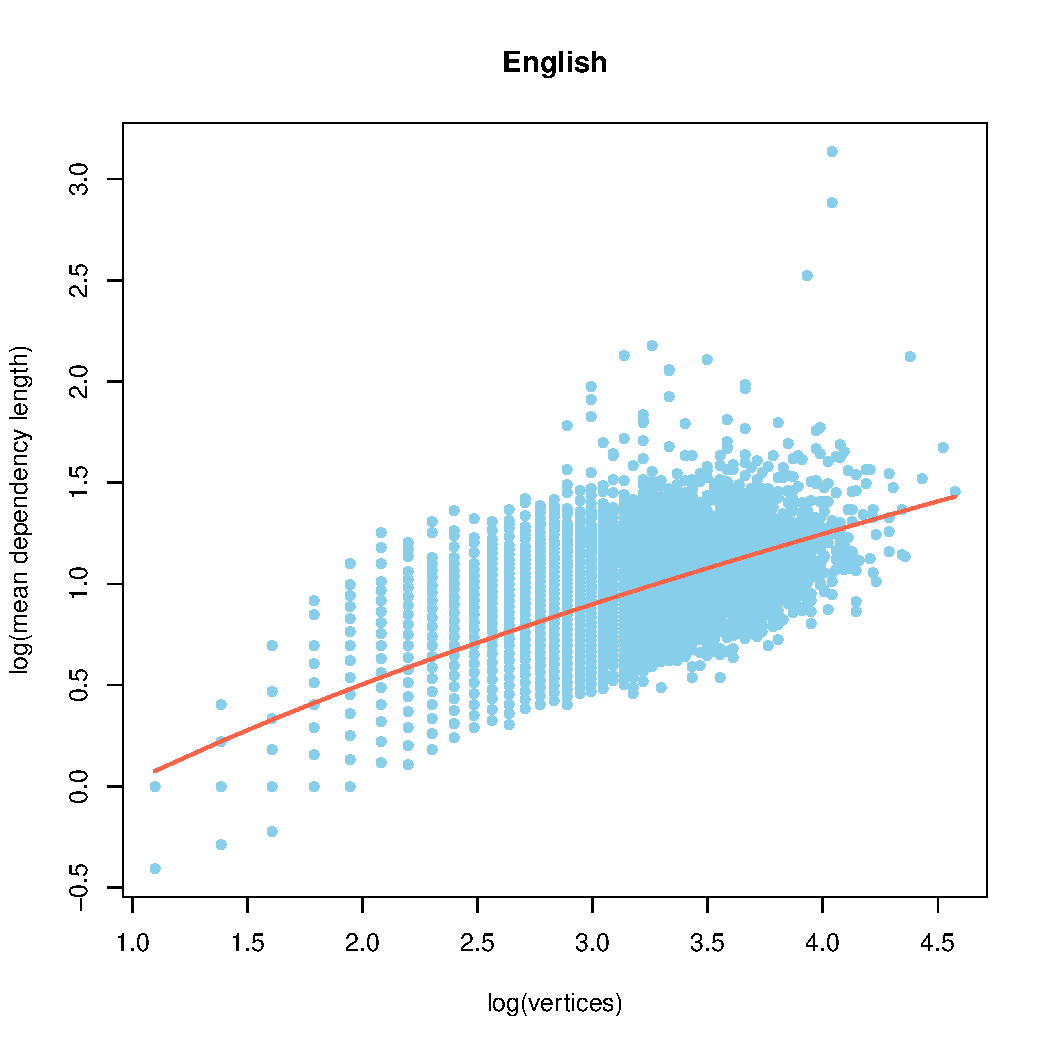
\includegraphics[scale=0.38]{English}}
	\caption{Plot of number of nodes versus mean edge length for different languages along with fitted curve following Model 2$+$}
	
\end{figure*}

\begin{figure*}[hbtp]
	\centering
	\subfigure[German Lnguage]{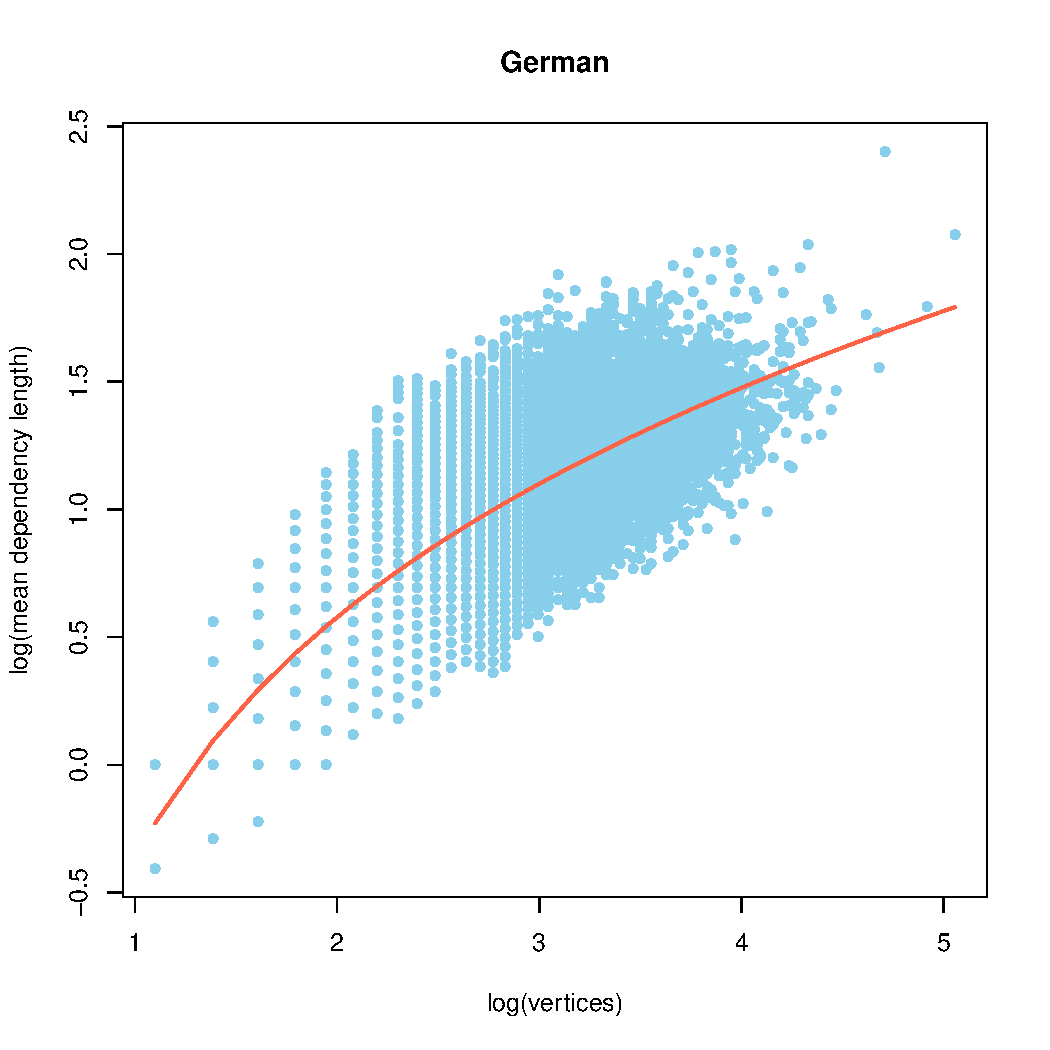
\includegraphics[scale=0.38]{German}}\quad
	\subfigure[Modern Greek Language]{\includegraphics[scale=0.38]{Greek_modern}}
	\caption{Plot of number of nodes versus mean edge length for different languages along with fitted curve following Model 2$+$}
	
\end{figure*}

\begin{figure*}[hbtp]
	\centering
	\subfigure[Hungarian Language]{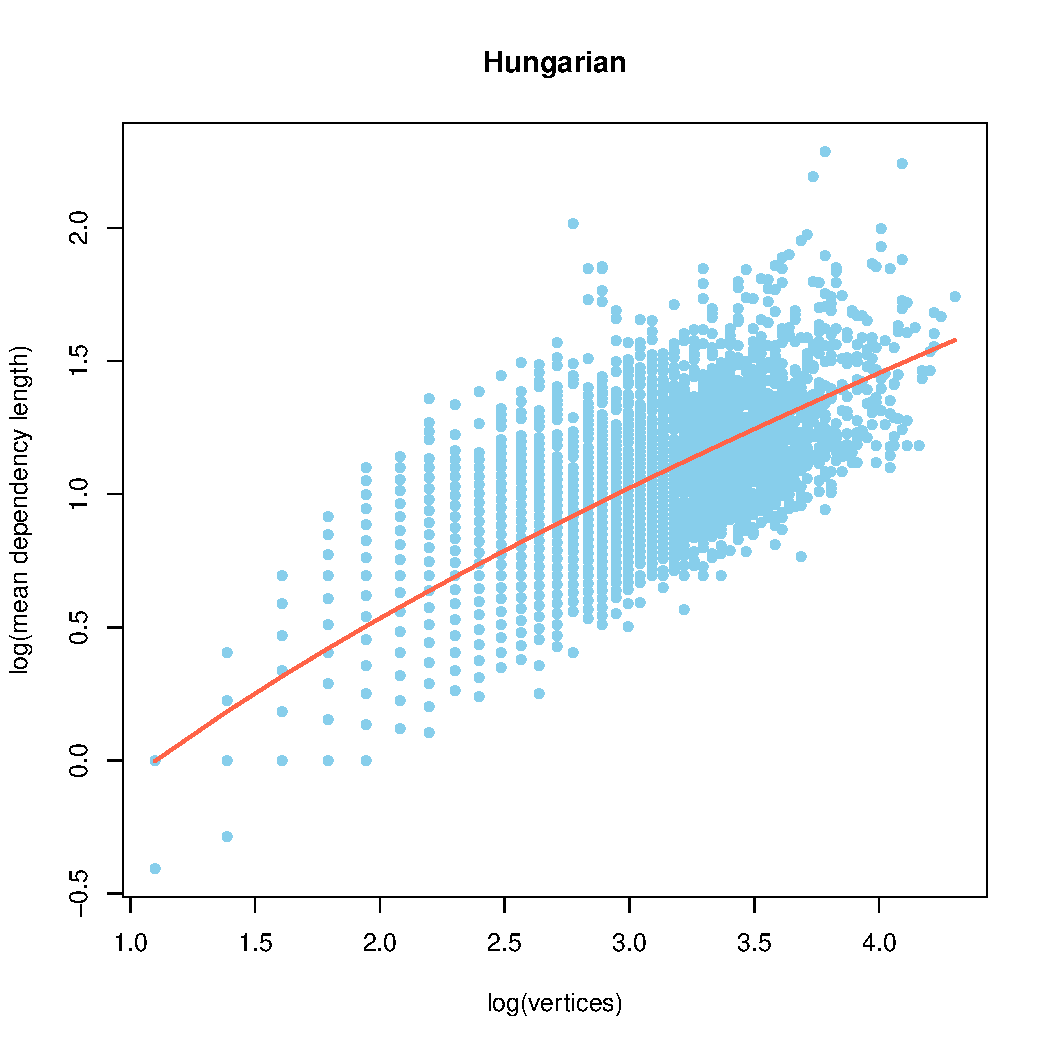
\includegraphics[scale=0.38]{Hungarian}}\quad
	\subfigure[Italian Language]{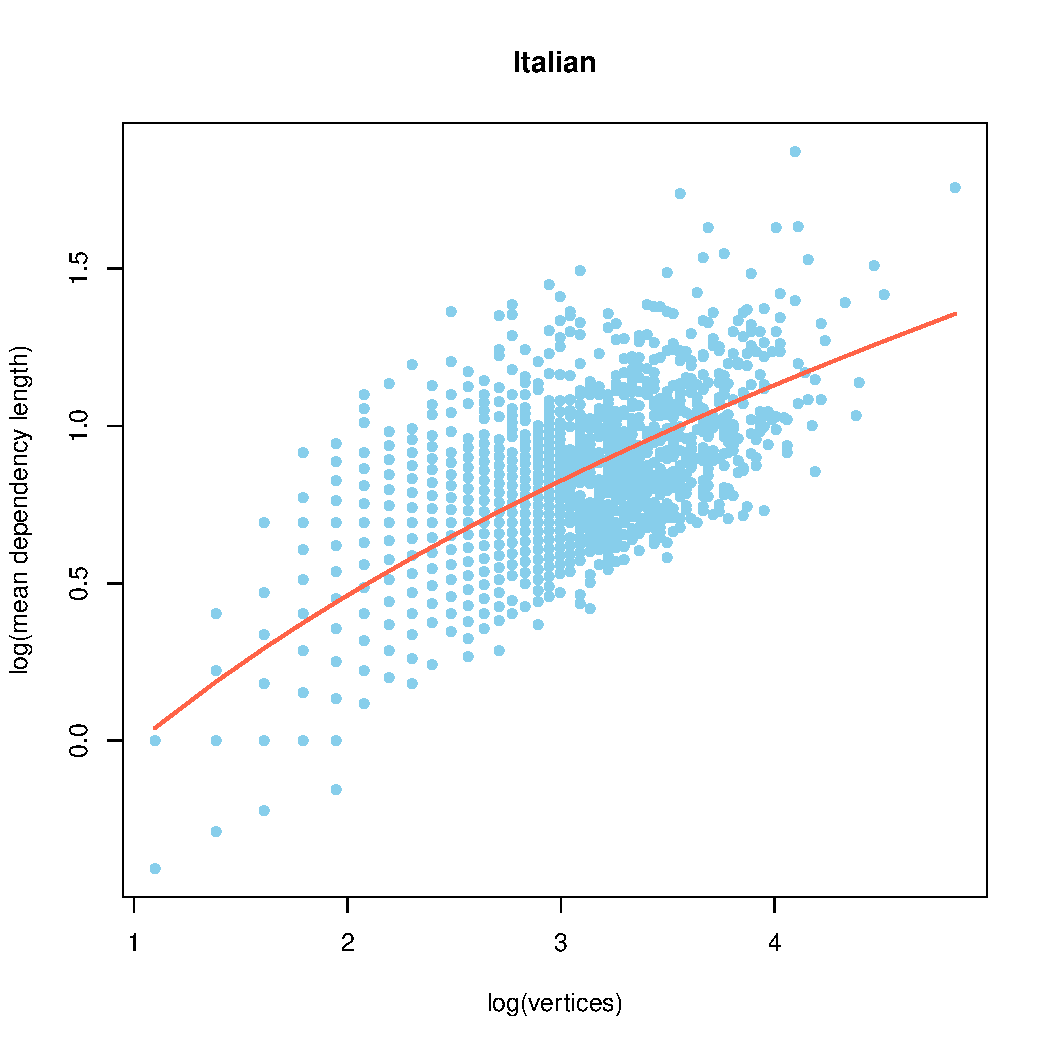
\includegraphics[scale=0.38]{Italian}}
	\caption{Plot of number of nodes versus mean edge length for different languages along with fitted curve following Model 2$+$}
	
\end{figure*}

\begin{figure*}[hbtp]
	\centering
	\subfigure[Japanese Language]{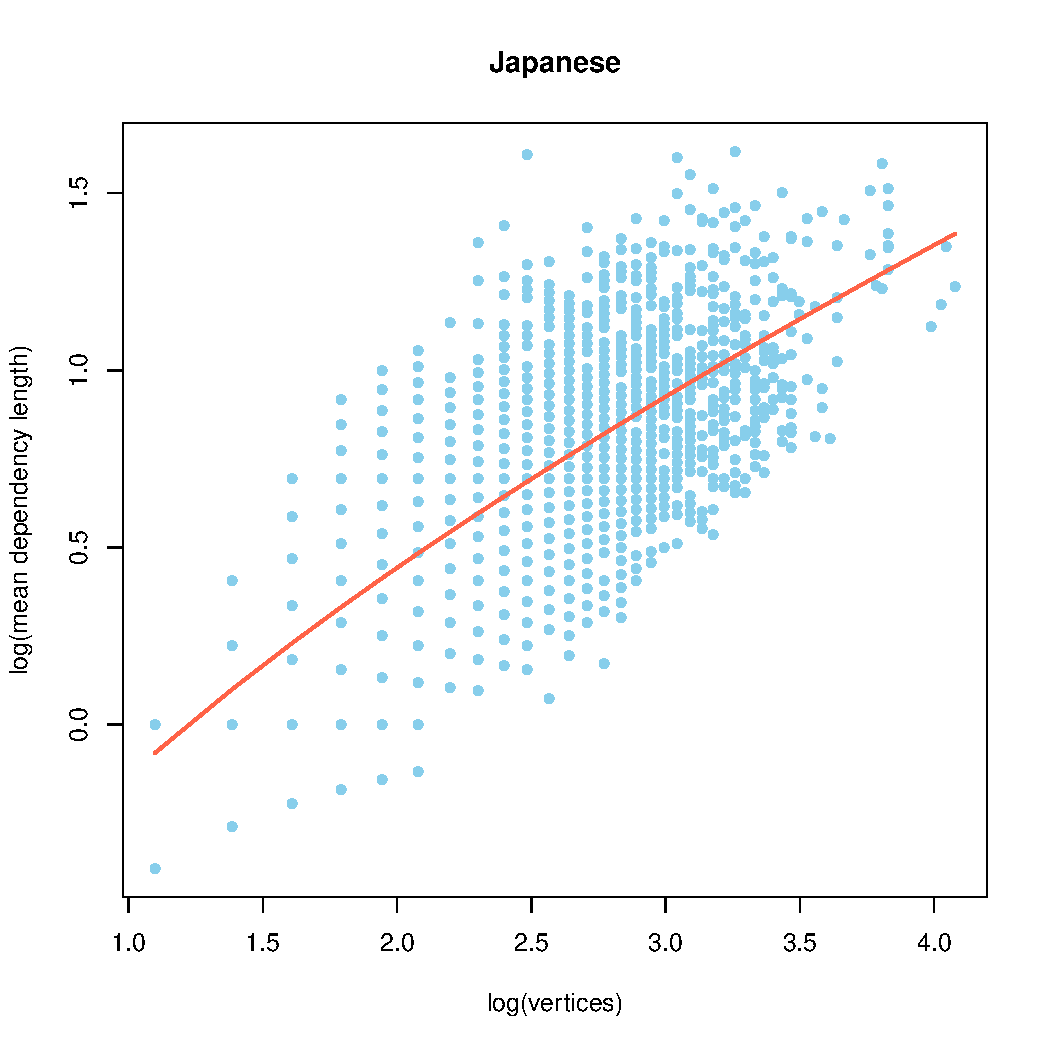
\includegraphics[scale=0.38]{Japanese}}\quad
	\subfigure[Latin Language]{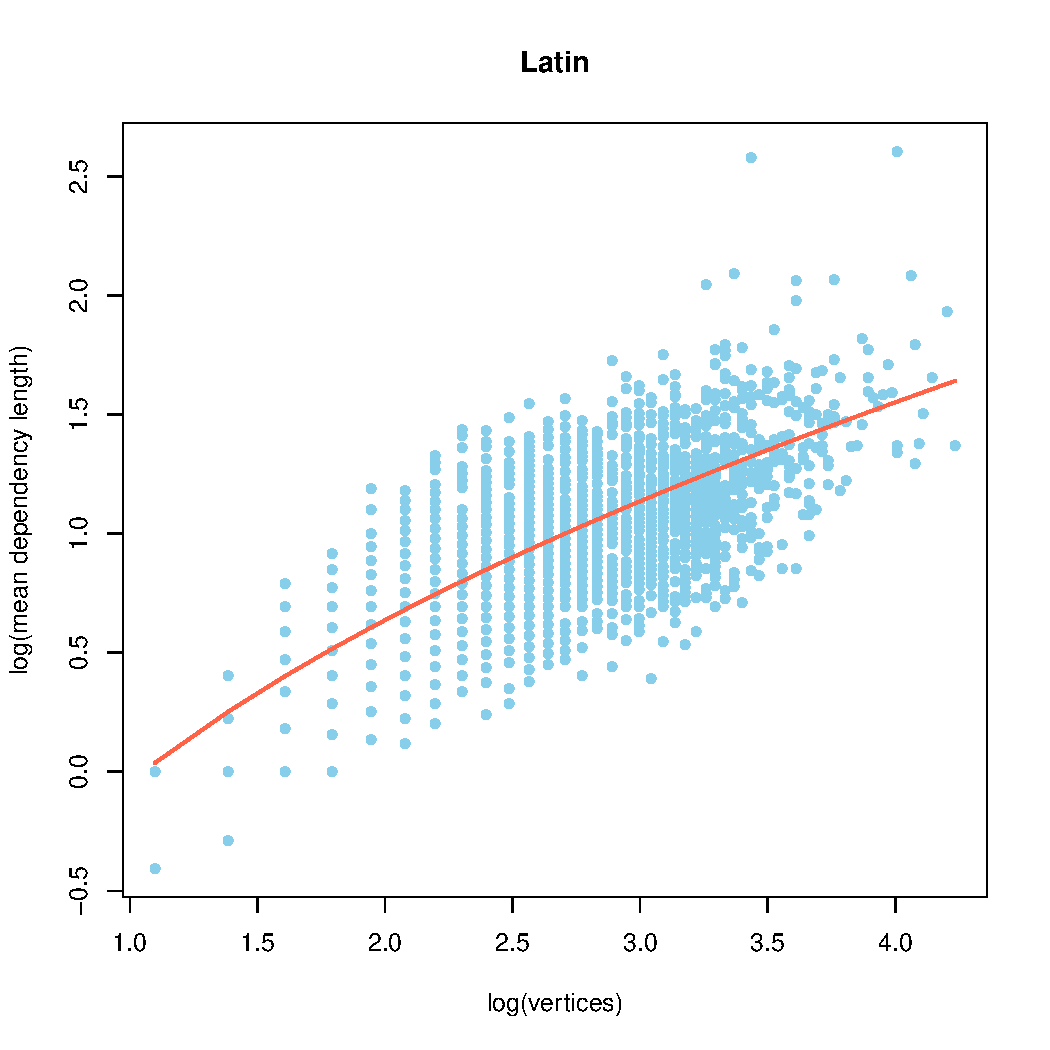
\includegraphics[scale=0.38]{Latin}}
	\caption{Plot of number of nodes versus mean edge length for different languages along with fitted curve following Model 2$+$}
	
\end{figure*}

\begin{figure*}[hbtp]
	\centering
	\subfigure[Persian Language]{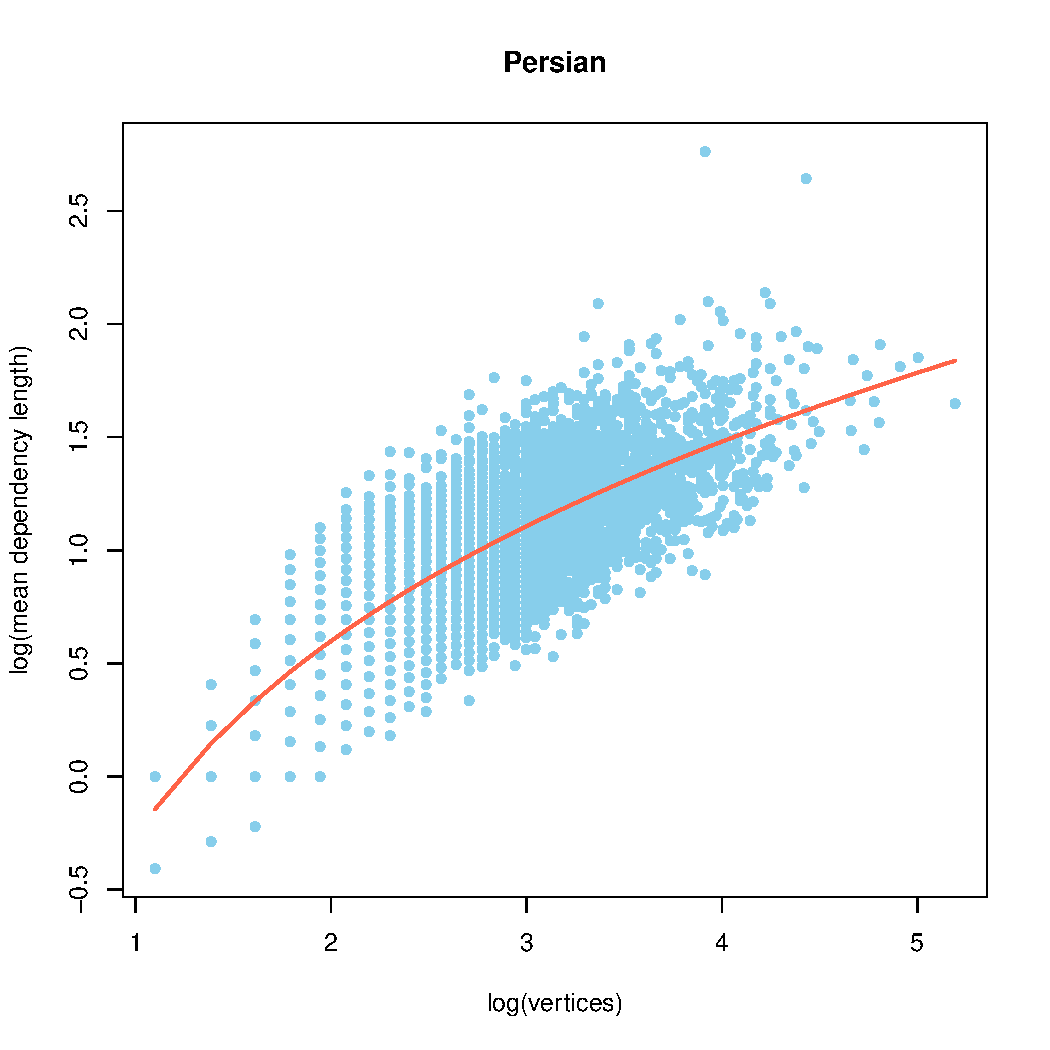
\includegraphics[scale=0.38]{Persian}}\quad
	\subfigure[Russian Language]{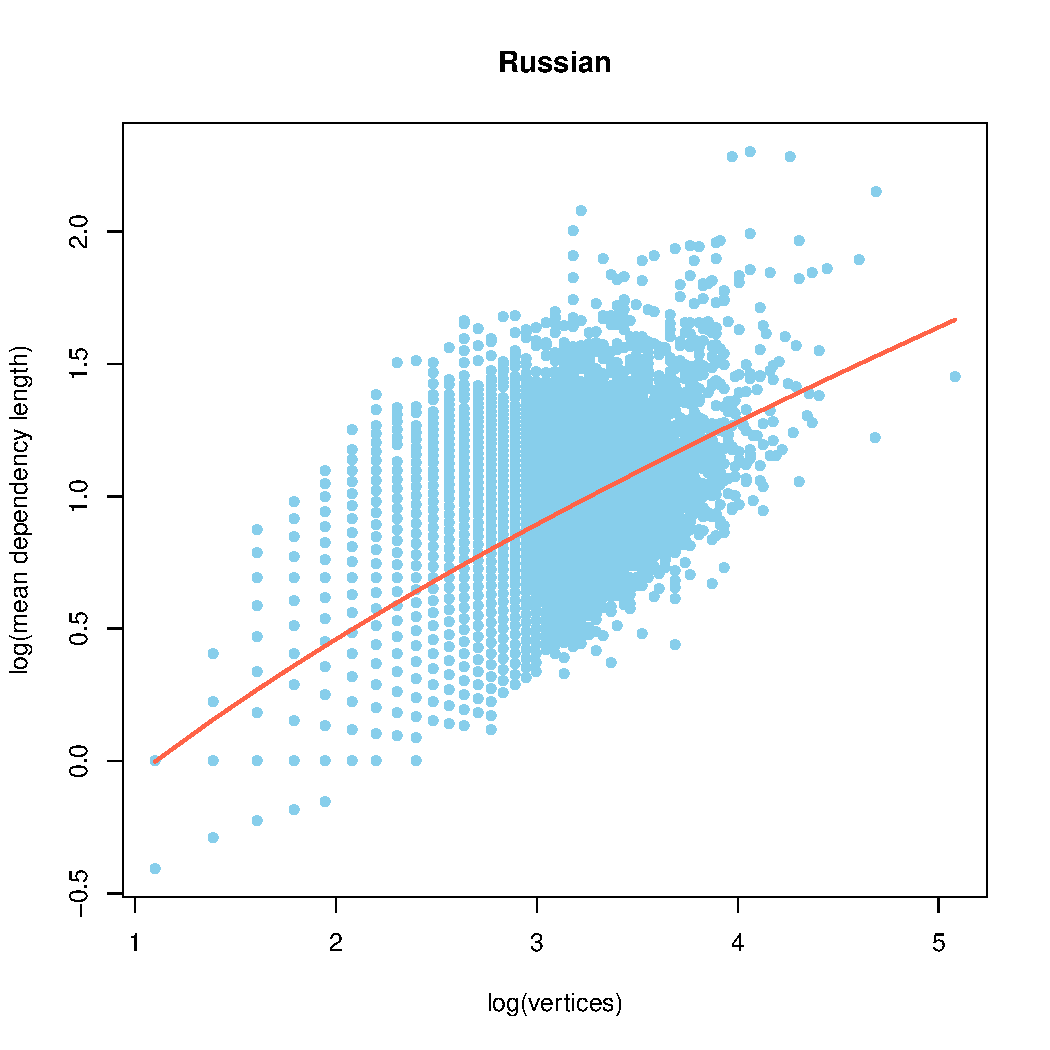
\includegraphics[scale=0.38]{Russian}}
	\caption{Plot of number of nodes versus mean edge length for different languages along with fitted curve following Model 2$+$}
	
\end{figure*}

\begin{figure*}[hbtp]
	\centering
	\subfigure[Slovak Language]{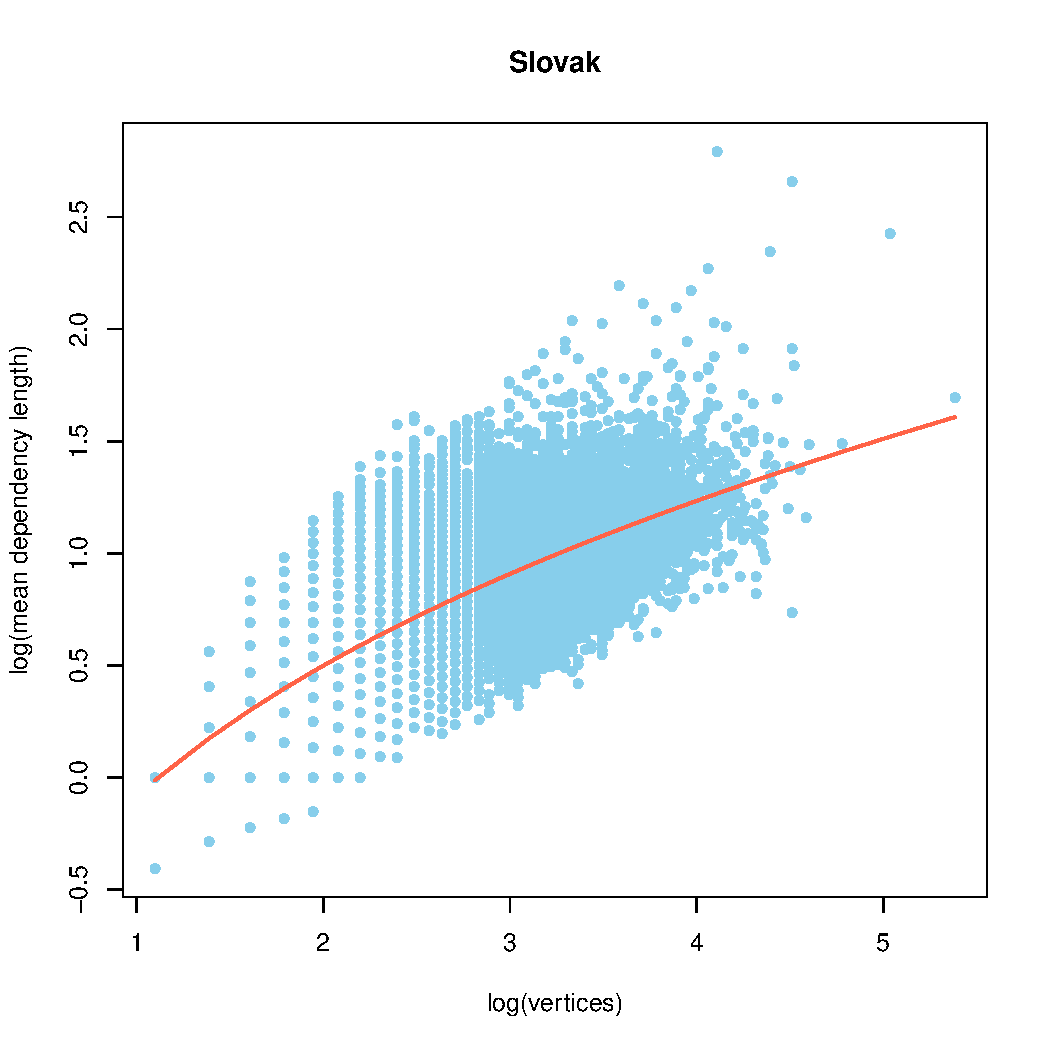
\includegraphics[scale=0.38]{Slovak}}\quad
	\subfigure[Slovene Language]{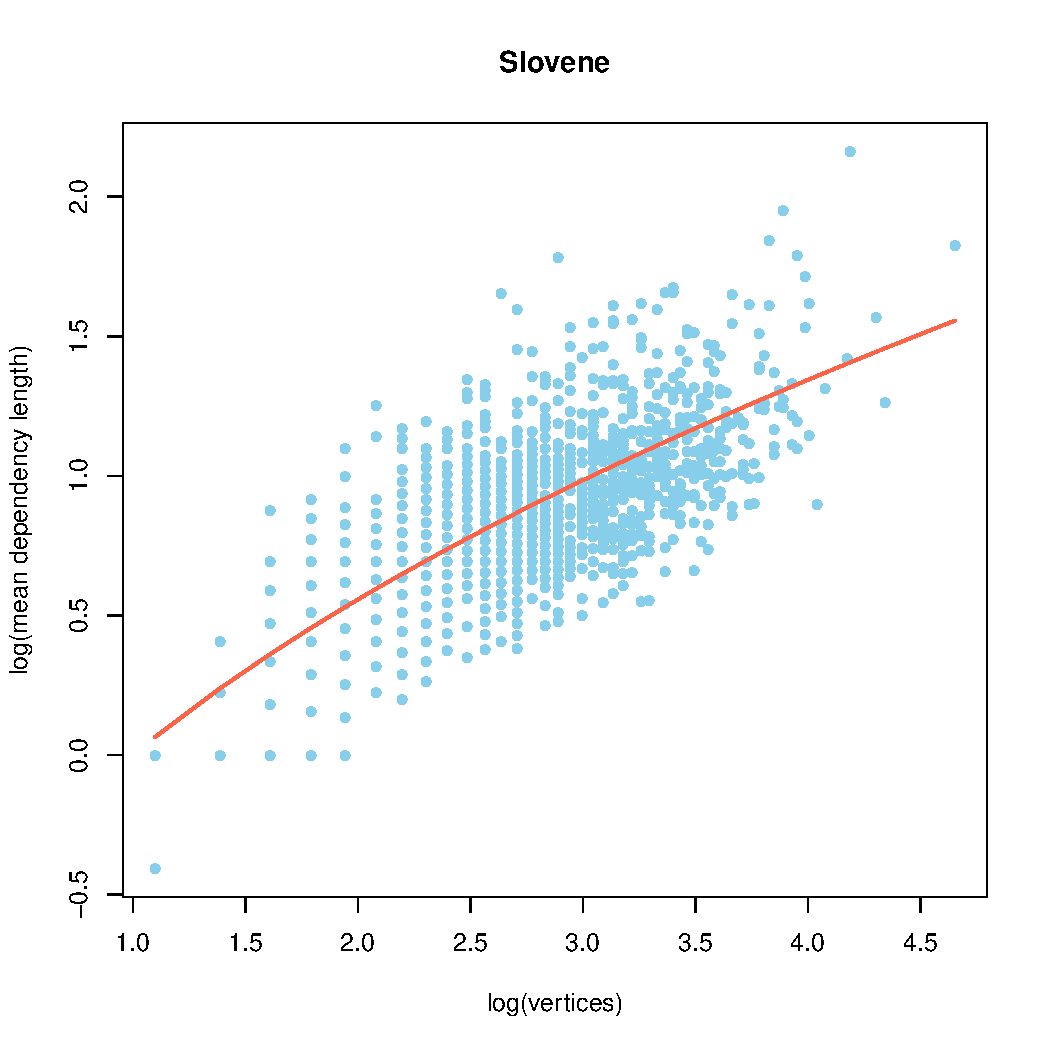
\includegraphics[scale=0.38]{Slovene}}
	\caption{Plot of number of nodes versus mean edge length for different languages along with fitted curve following Model 2$+$}
	
\end{figure*}

\begin{figure*}[hbtp]
	\centering
	\subfigure[Spanish Language]{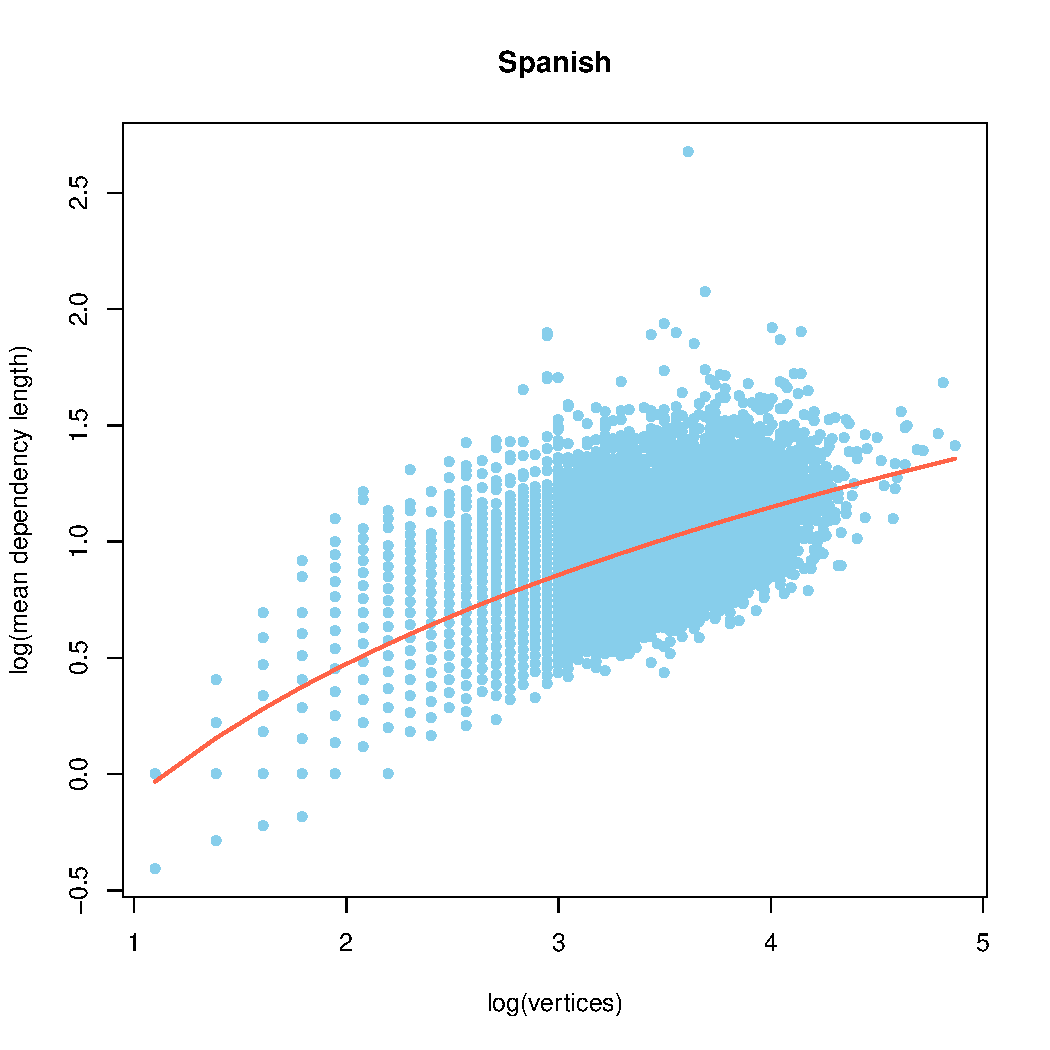
\includegraphics[scale=0.38]{Spanish}}\quad
	\subfigure[Swedish Language]{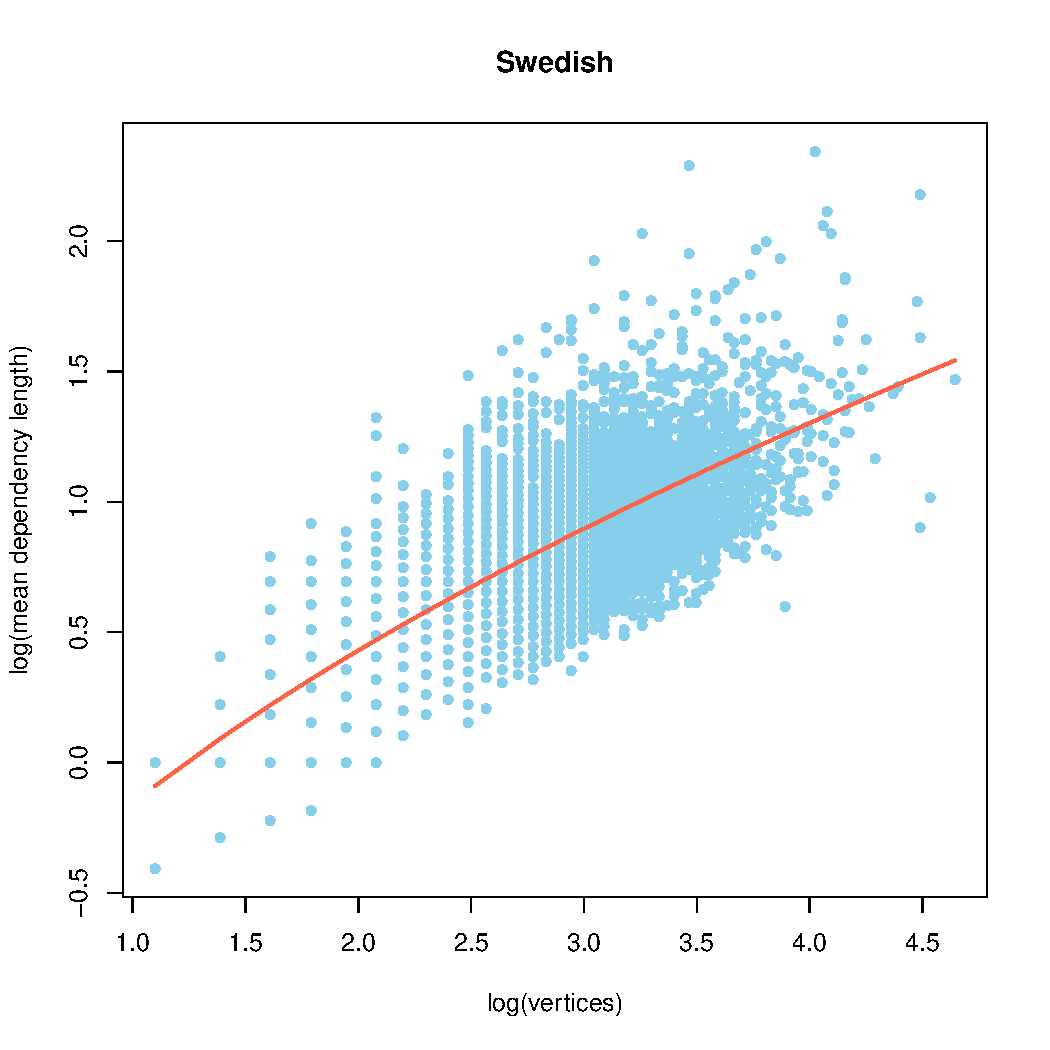
\includegraphics[scale=0.38]{Swedish}}
	\subfigure[Turkish Language]{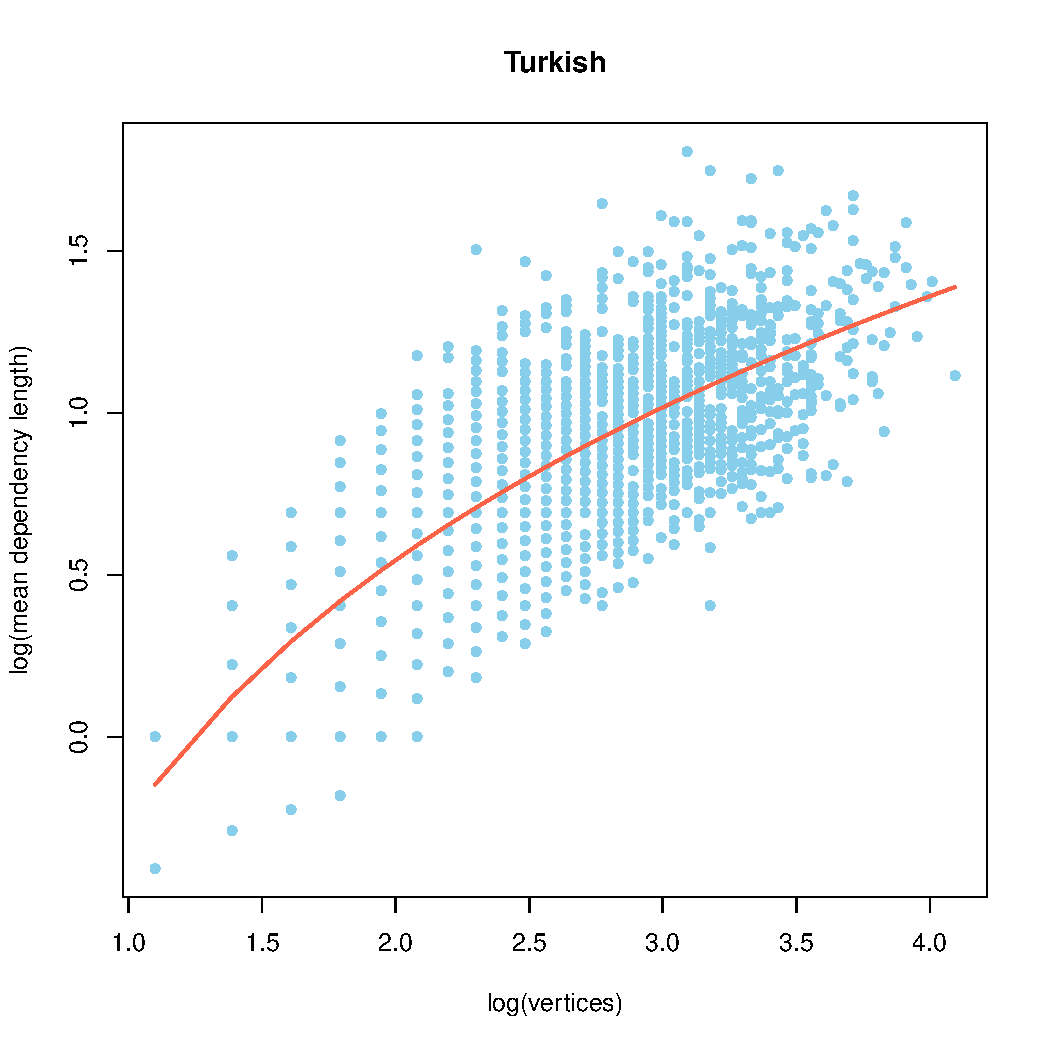
\includegraphics[scale=0.38]{Turkish}}
	\caption{Plot of number of nodes versus mean edge length for different languages along with fitted curve following Model 2$+$}
	
\end{figure*}


\begin{figure}[hbtp]
	\centering
	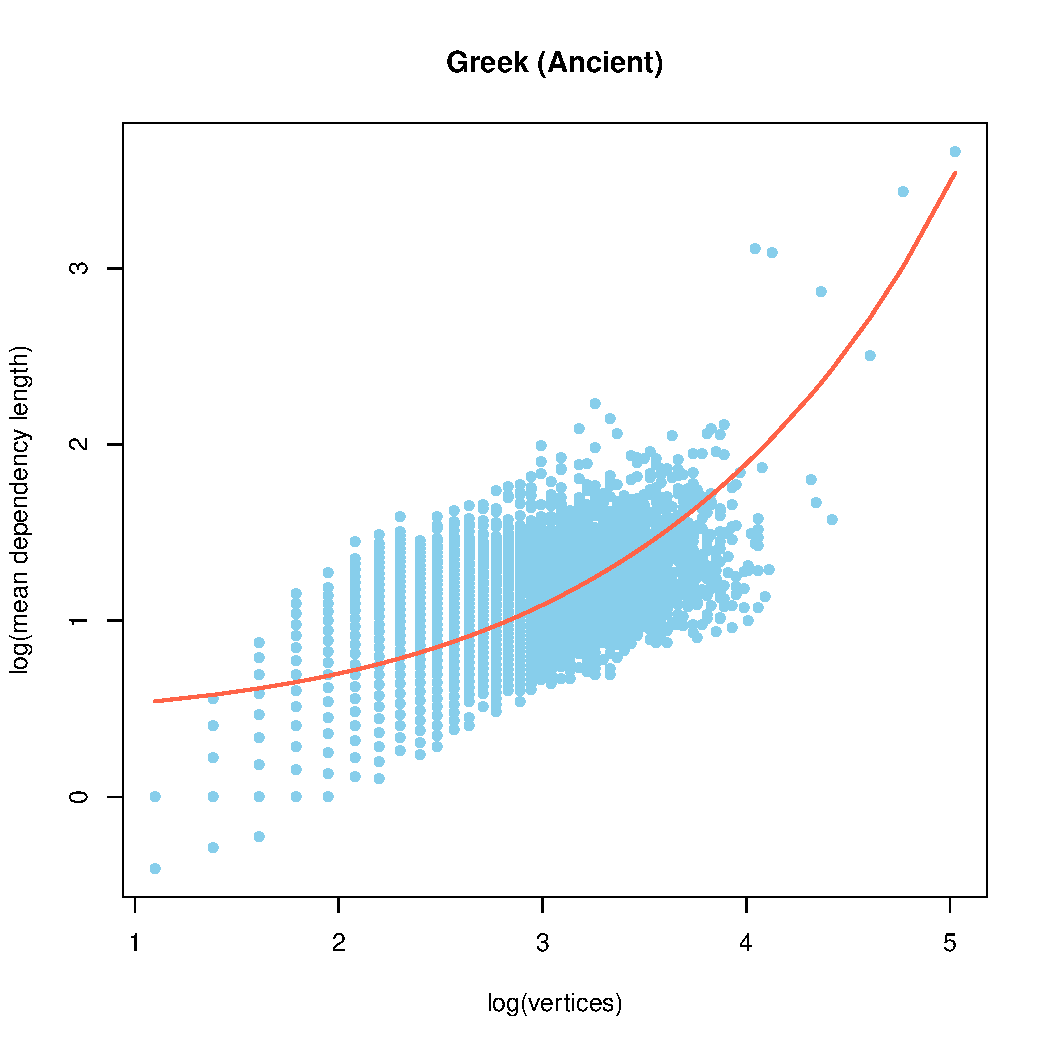
\includegraphics[scale=0.38]{Greek_Ancient}
	\label{Ancient Greek Language}
	\caption{Plot of number of nodes versus mean edge length for \textbf{Ancient Greek Language} along with fitted curve following Model 3$+$}
\end{figure}

\begin{figure*}[hbtp]
	\centering
	\subfigure[Bengali Language]{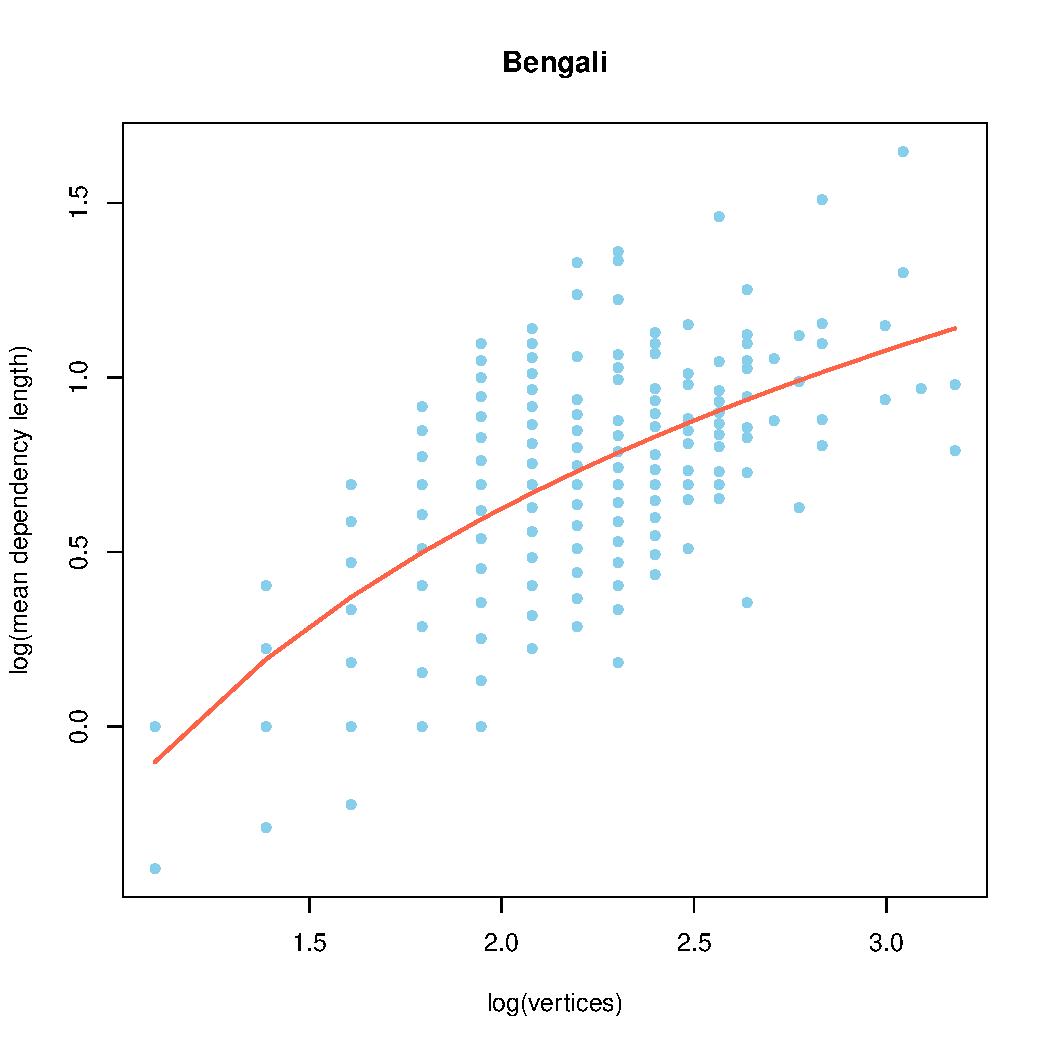
\includegraphics[scale=0.38]{Bengali}}\quad
	\subfigure[Danish Language]{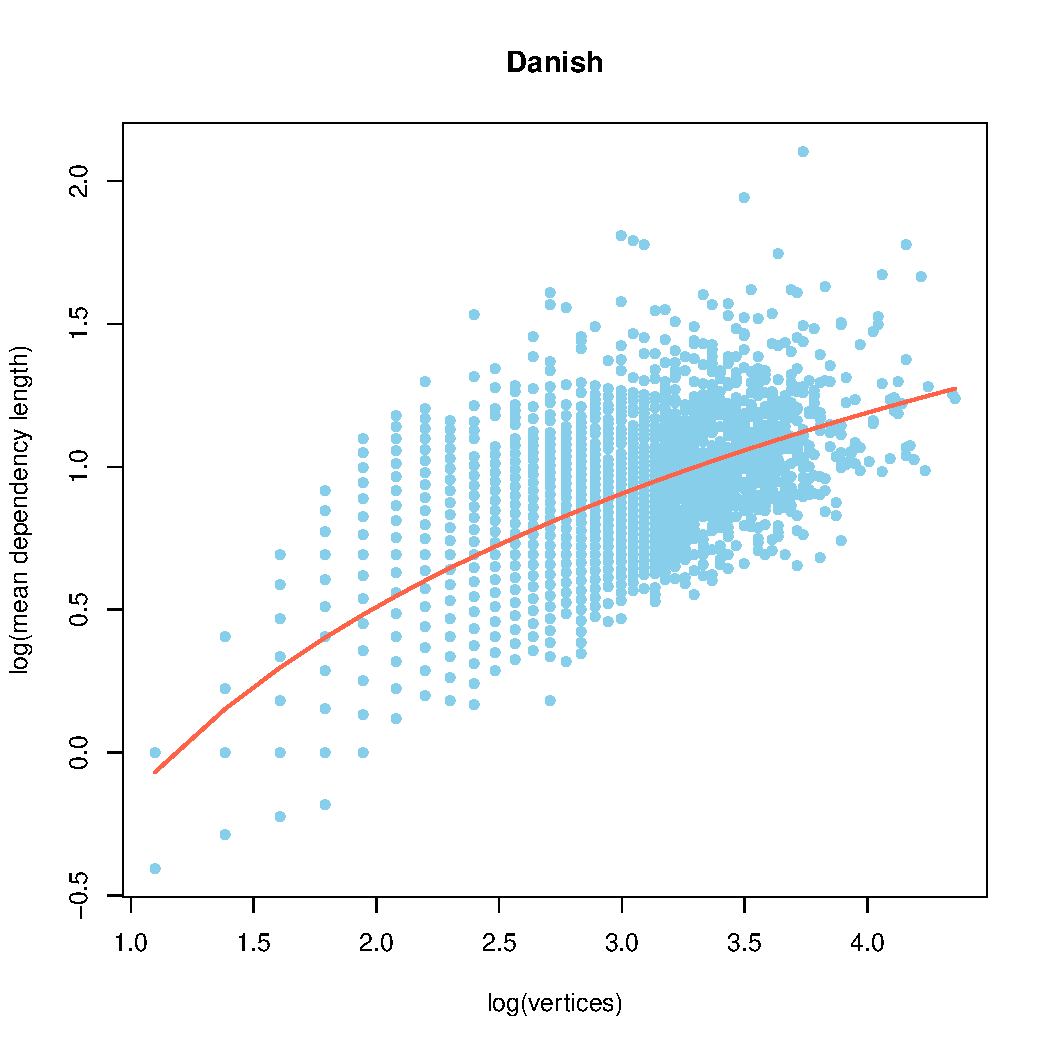
\includegraphics[scale=0.38]{Danish}}
	\caption{Plot of number of nodes versus mean edge length for different languages along with fitted curve following Model 4$+$}
	
\end{figure*}

\begin{figure*}[hbtp]
	\centering
	\subfigure[Dutch Language]{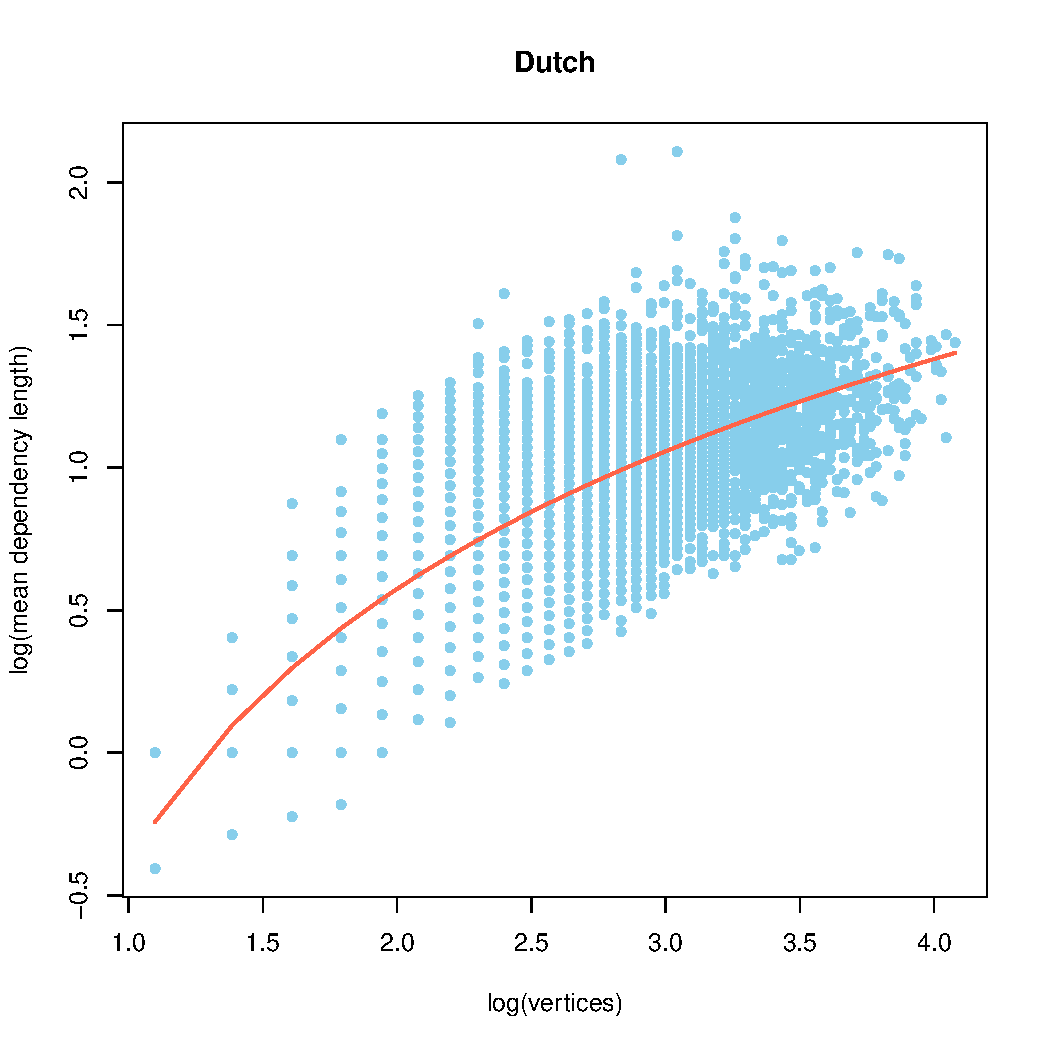
\includegraphics[scale=0.38]{Dutch}}\quad
	\subfigure[Estonian Language]{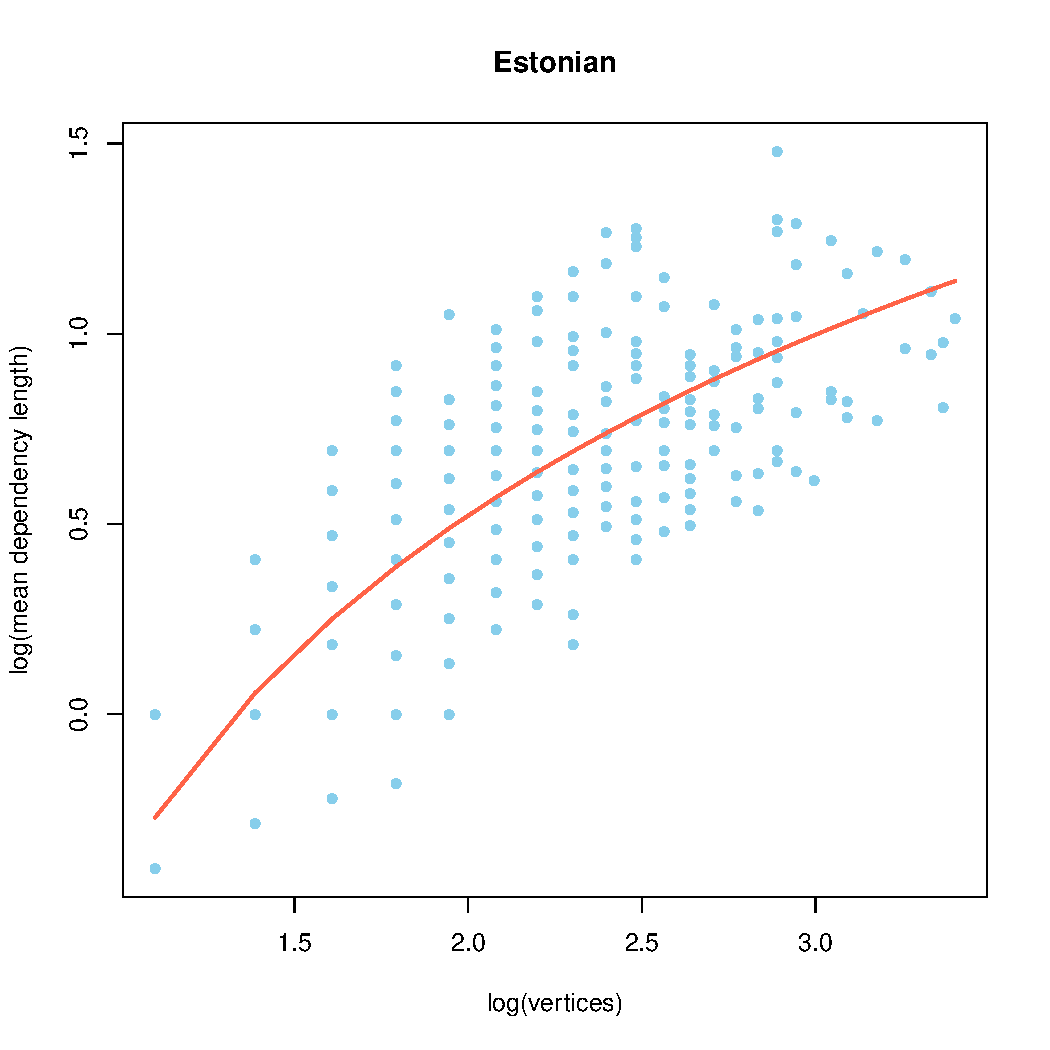
\includegraphics[scale=0.38]{Estonian}}
	\caption{Plot of number of nodes versus mean edge length for different languages along with fitted curve following Model 4$+$}
	
\end{figure*}

\begin{figure*}[hbtp]
	\centering
	\subfigure[Finnish Language]{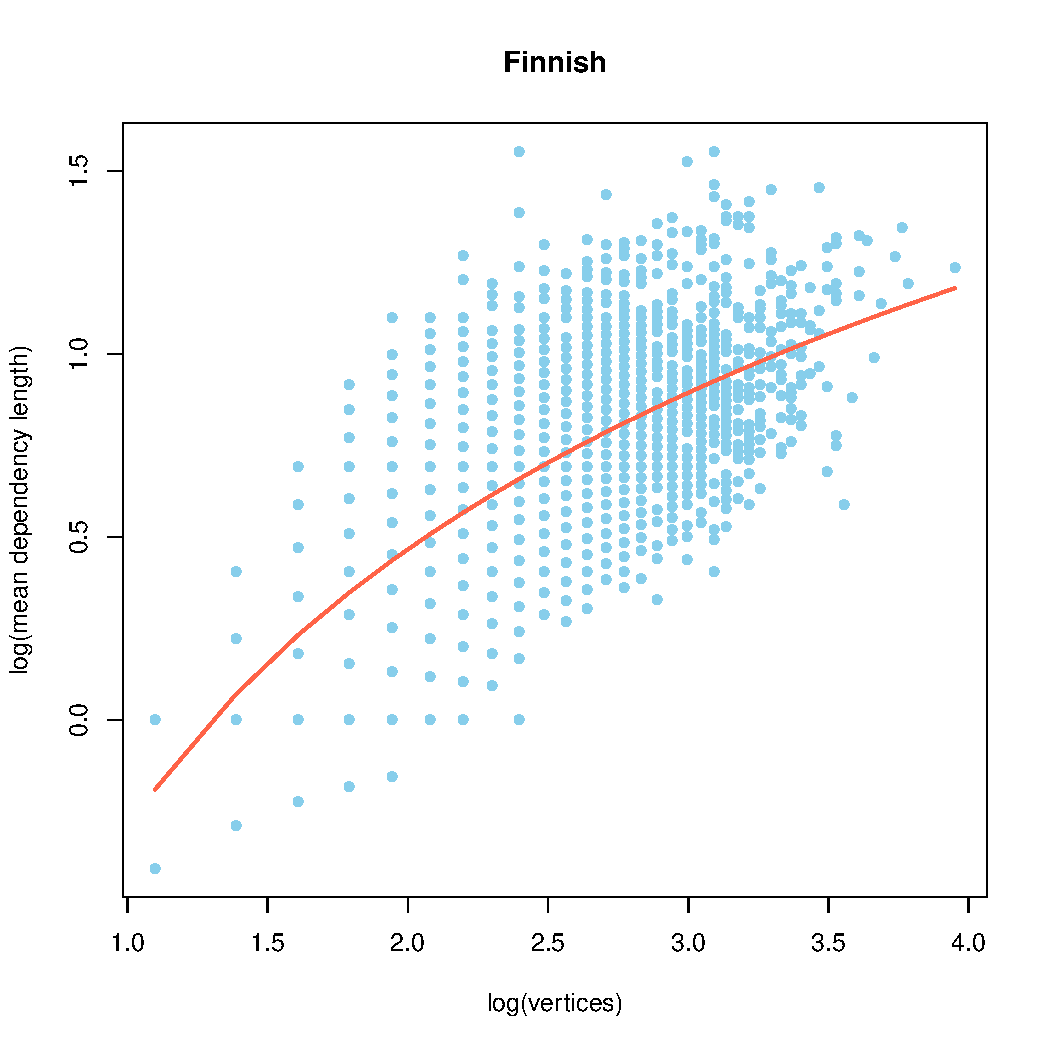
\includegraphics[scale=0.38]{Finnish}}\quad
	\subfigure[Hindi Language]{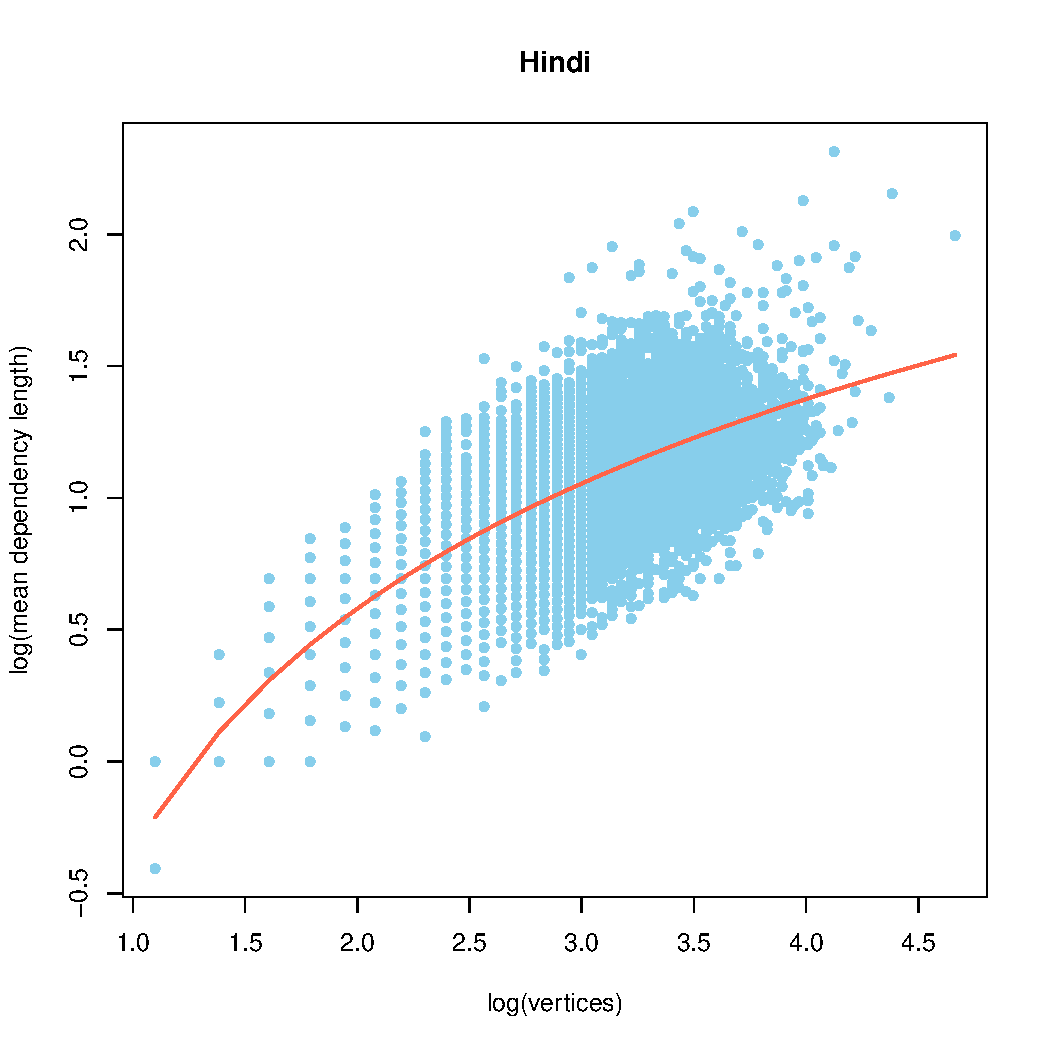
\includegraphics[scale=0.38]{Hindi}}
	\caption{Plot of number of nodes versus mean edge length for different languages along with fitted curve following Model 4$+$}
	
\end{figure*}

\begin{figure*}[hbtp]
	\centering
	\subfigure[Portuguese Language]{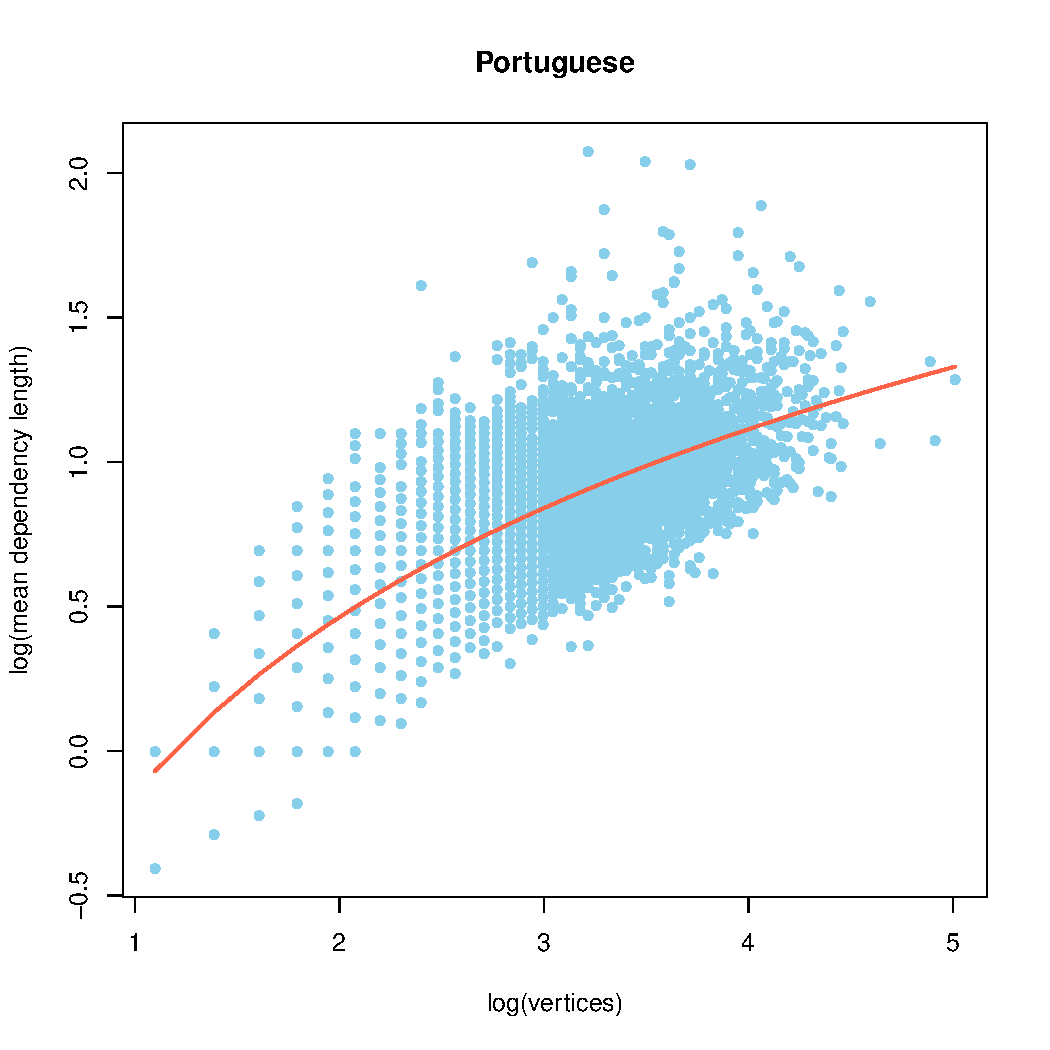
\includegraphics[scale=0.38]{Portuguese}}\quad
	\subfigure[Romanian Language]{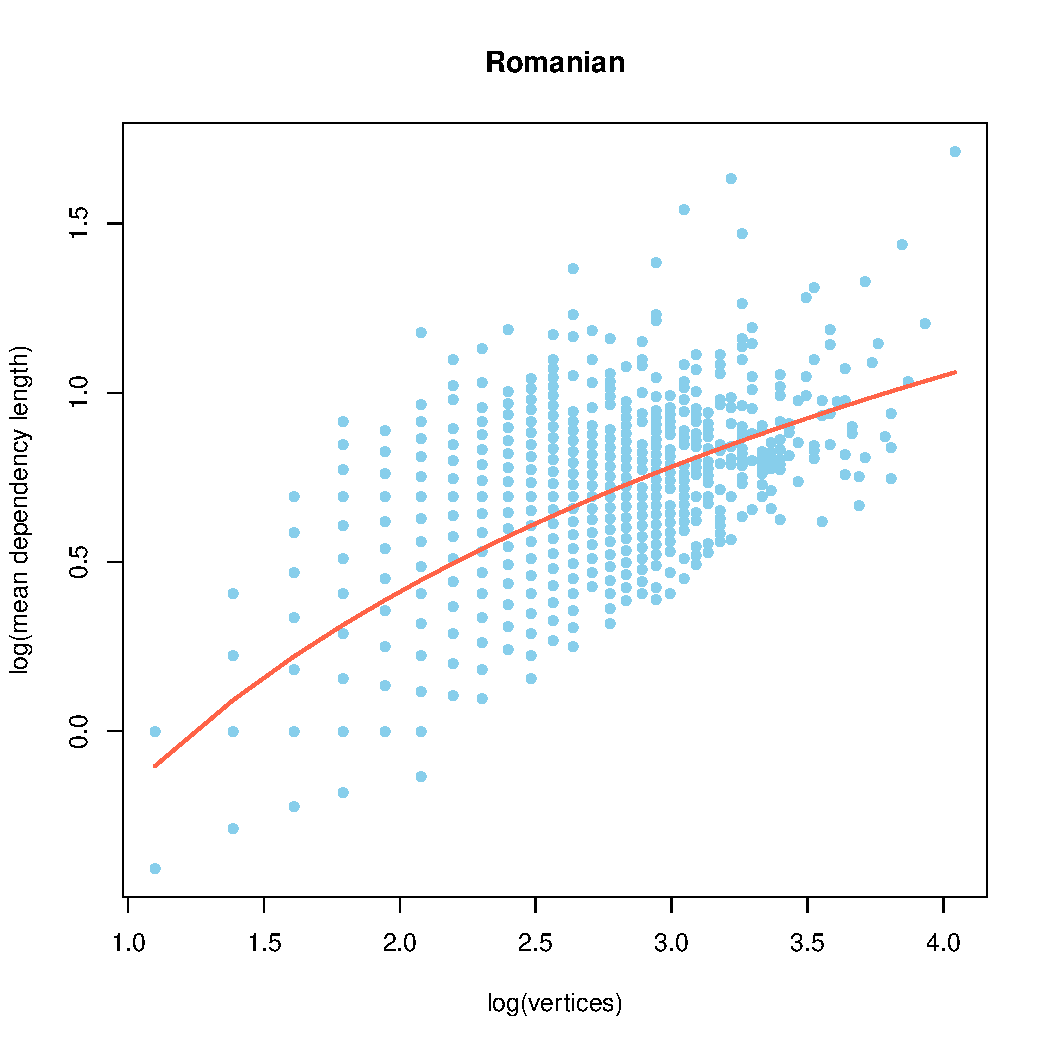
\includegraphics[scale=0.38]{Romanian}}
	\subfigure[Telugu Language]{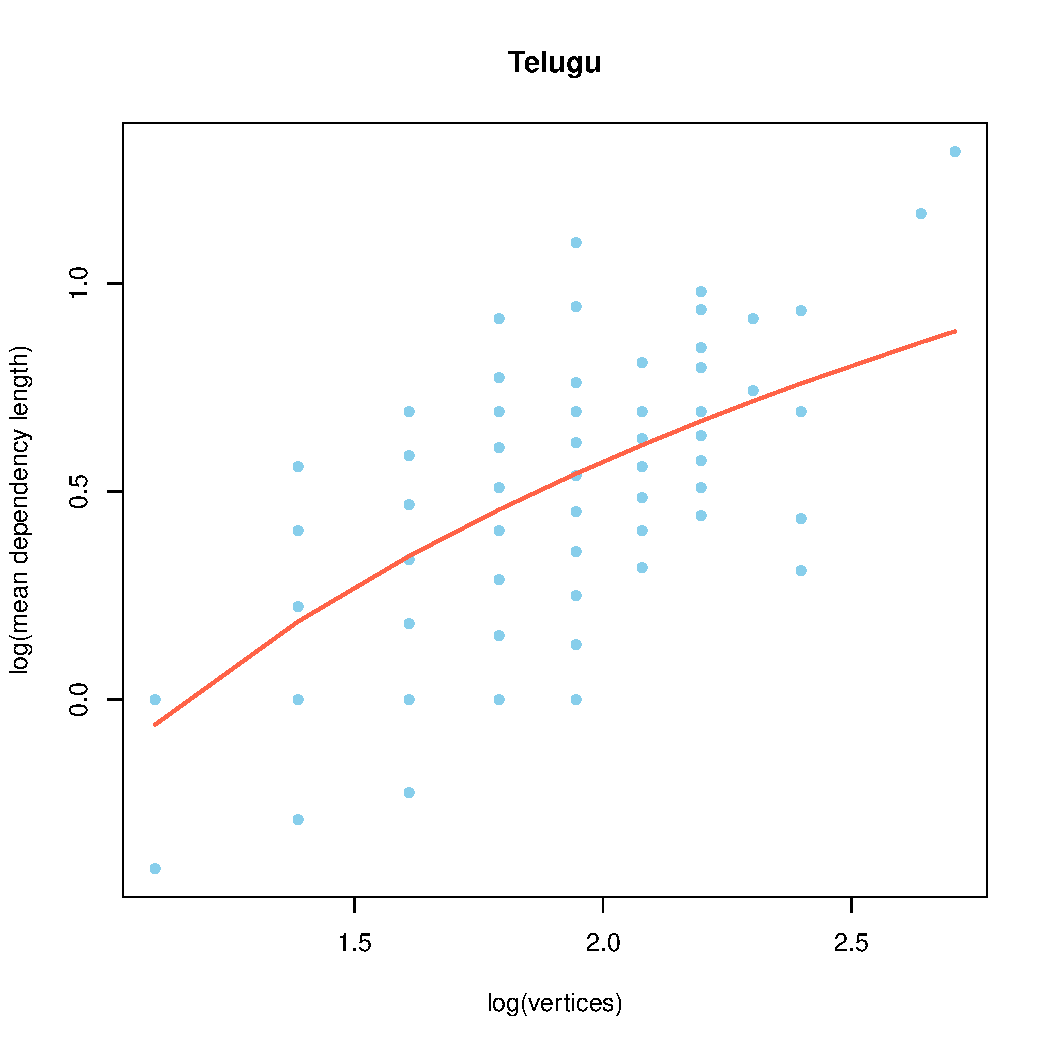
\includegraphics[scale=0.38]{Telugu}}
	\caption{Plot of number of nodes versus mean edge length for different languages along with fitted curve following Model 4$+$}
\end{figure*}


\begin{figure*}[hbtp]
	\centering
	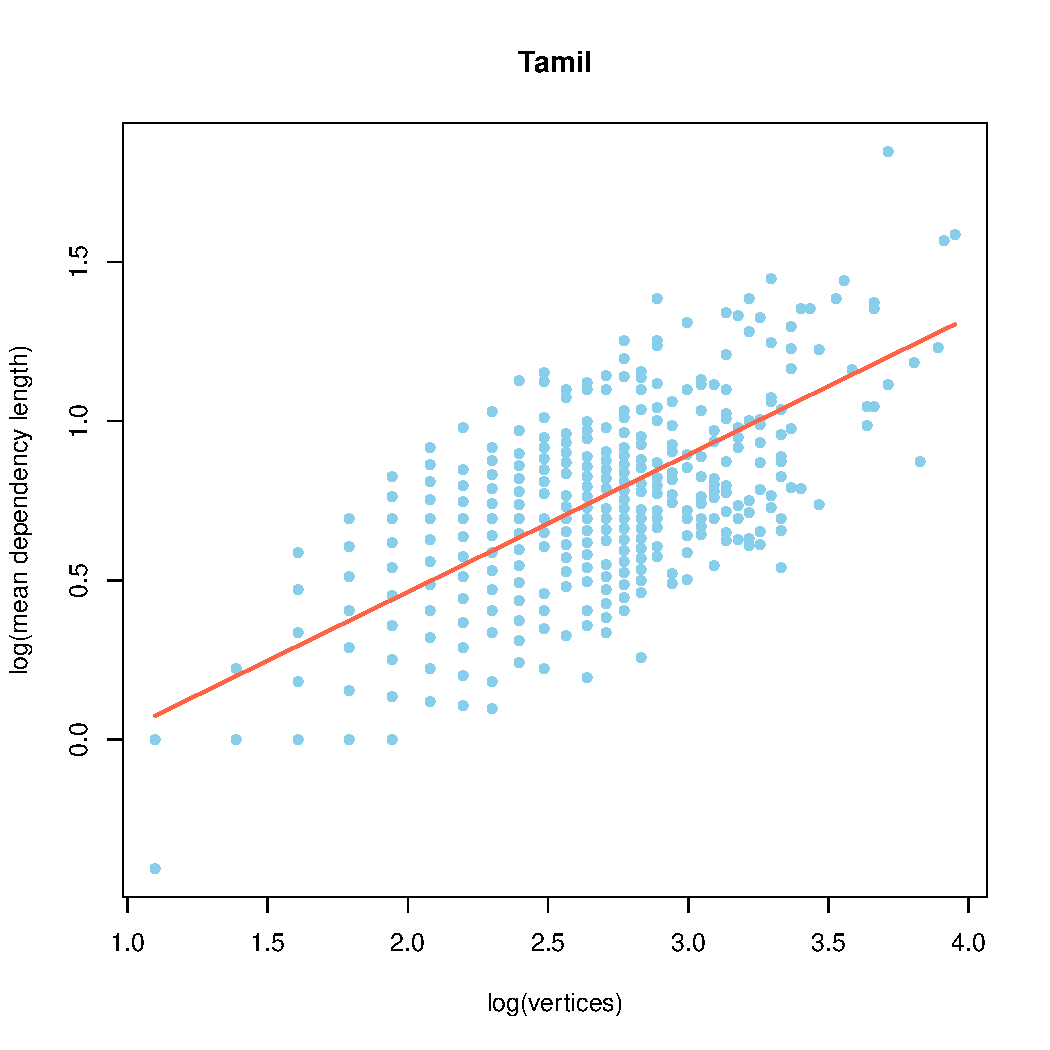
\includegraphics[scale=0.38]{Tamil}
	\label{Tamil Language}
	\caption{Tamil Language}
	\caption{Plot of number of nodes versus mean edge length for \textbf{Tamil Language} along with a curve following Model 2}
\end{figure*}


\begin{table}[hbtp]
	\centering
	\begin{tabular}{rlrrrrr}
		\hline
		& Language & $N$ & $\mu_N$ & $\sigma_N$ & $\mu_x$ & $\sigma_x$ \\ 
		\hline
		1 & Arabic & 2333.00 & 25.81 & 21.08 & 2.25 & 0.96 \\ 
		2 & Basque & 9757.00 & 11.22 & 5.42 & 1.84 & 0.61 \\ 
		3 & Bengali & 926.00 & 6.52 & 3.07 & 1.63 & 0.60 \\ 
		4 & Bulgarian & 12809.00 & 13.06 & 7.70 & 1.93 & 0.60 \\ 
		5 & Catalan & 14719.00 & 26.63 & 13.97 & 2.46 & 0.68 \\ 
		6 & Czech & 78463.00 & 15.86 & 8.98 & 2.11 & 0.70 \\ 
		7 & Danish & 5207.00 & 16.37 & 10.03 & 2.15 & 0.70 \\ 
		8 & Dutch & 11841.00 & 12.88 & 8.36 & 2.17 & 0.85 \\ 
		9 & English & 18612.00 & 21.41 & 10.09 & 2.43 & 0.75 \\ 
		10 & Estonian & 1281.00 & 6.18 & 3.69 & 1.38 & 0.56 \\ 
		11 & German & 35887.00 & 16.26 & 9.62 & 2.54 & 0.95 \\ 
		12 & Greek (Modern) & 2637.00 & 22.61 & 12.75 & 2.33 & 0.70 \\ 
		13 & Greek (Ancient) & 19913.00 & 12.78 & 7.90 & 2.43 & 0.95 \\ 
		14 & Finnish & 4251.00 & 11.83 & 5.74 & 1.90 & 0.58 \\ 
		15 & Hindi & 12471.00 & 20.33 & 9.28 & 2.77 & 0.77 \\ 
		16 & Hungarian & 6299.00 & 18.56 & 10.59 & 2.55 & 0.92 \\ 
		17 & Italian & 2630.00 & 17.88 & 11.93 & 2.07 & 0.64 \\ 
		18 & Japanese & 7213.00 & 7.87 & 6.09 & 1.48 & 0.65 \\ 
		19 & Latin & 3227.00 & 14.23 & 8.91 & 2.49 & 1.00 \\ 
		20 & Persian & 12324.00 & 13.83 & 10.85 & 2.31 & 0.96 \\ 
		21 & Portuguese & 8992.00 & 20.23 & 13.06 & 2.17 & 0.67 \\ 
		22 & Romanian & 3708.00 & 9.59 & 6.27 & 1.56 & 0.51 \\ 
		23 & Russian & 33479.00 & 14.73 & 8.76 & 2.04 & 0.73 \\ 
		24 & Slovak & 52208.00 & 13.37 & 9.11 & 1.98 & 0.70 \\ 
		25 & Slovene & 1860.00 & 15.18 & 10.24 & 2.24 & 0.82 \\ 
		26 & Spanish & 15697.00 & 26.59 & 14.04 & 2.45 & 0.69 \\ 
		27 & Swedish & 11069.00 & 15.81 & 9.01 & 2.10 & 0.71 \\ 
		28 & Tamil & 599.00 & 14.32 & 7.50 & 2.05 & 0.66 \\ 
		29 & Telugu & 1095.00 & 4.15 & 1.52 & 1.19 & 0.38 \\ 
		30 & Turkish & 4682.00 & 10.37 & 7.84 & 1.85 & 0.81 \\ 
		\hline
	\end{tabular}
\caption{Summary of the properties of the degree sequences. $N$ is the sample size (the number of sentences or dependency trees), $\mu_N$ and $\sigma_N$ are, respectively, the mean and the standard deviation of n, the sentence length (n is the number of vertices of a trees), $\mu_x$ and $\sigma_x$ are the mean and the standard deviation of the target metric
i.e. mean edge length in syntactic dependency trees}
\end{table}




\begin{table}[hbtp]
\captionsetup{justification=raggedright}
\caption {Values of best parameters for Model 1 and 2 (all variants)}
\centering
\begin{tabular}{rlrrrrrrrr}
  \hline
 & Language & 1(b) & 1+(b) & 1+(d) & 2(a) & 2(b) & 2+(a) & 2+(b) & 2+(d) \\ 
  \hline
1 & Arabic & 0.35 & 0.38 & -0.19 & 0.65 & 0.41 & 1.56 & 0.27 & -1.23 \\ 
  2 & Basque & 0.38 & 0.45 & -0.26 & 0.56 & 0.51 & 2.77 & 0.21 & -2.65 \\ 
  3 & Bengali & 0.47 & 0.54 & -0.22 & 0.54 & 0.60 & 321.44 & 0.00 & -321.54 \\ 
  4 & Bulgarian & 0.38 & 0.39 & -0.07 & 0.72 & 0.40 & 3.64 & 0.15 & -3.32 \\ 
  5 & Catalan & 0.36 & 0.36 & 0.03 & 0.80 & 0.35 & 1.25 & 0.28 & -0.60 \\ 
  6 & Czech & 0.38 & 0.40 & -0.08 & 0.71 & 0.41 & 3.17 & 0.17 & -2.87 \\ 
  7 & Danish & 0.39 & 0.38 & 0.01 & 0.79 & 0.38 & 36.09 & 0.02 & -35.99 \\ 
  8 & Dutch & 0.45 & 0.47 & -0.10 & 0.67 & 0.48 & 103.24 & 0.01 & -103.63 \\ 
  9 & English & 0.39 & 0.38 & 0.03 & 0.80 & 0.37 & 1.85 & 0.24 & -1.32 \\ 
  10 & Estonian & 0.38 & 0.50 & -0.33 & 0.49 & 0.59 & 24.67 & 0.02 & -24.33 \\ 
  11 & German & 0.47 & 0.48 & -0.08 & 0.68 & 0.49 & 8.02 & 0.11 & -8.30 \\ 
  12 & Greek (Modern) & 0.36 & 0.36 & 0.00 & 0.79 & 0.36 & 3.02 & 0.17 & -2.64 \\ 
  13 & Greek (Ancient) & 0.50 & 0.49 & 0.04 & 0.74 & 0.49 & 0.58 & 0.54 & 0.25 \\ 
  14 & Finnish & 0.38 & 0.42 & -0.14 & 0.65 & 0.44 & 21.28 & 0.04 & -21.31 \\ 
  15 & Hindi & 0.45 & 0.42 & 0.19 & 0.88 & 0.39 & 108.35 & 0.01 & -108.21 \\ 
  16 & Hungarian & 0.44 & 0.45 & -0.09 & 0.68 & 0.47 & 1.41 & 0.33 & -1.03 \\ 
  17 & Italian & 0.35 & 0.35 & 0.01 & 0.80 & 0.35 & 3.20 & 0.15 & -2.74 \\ 
  18 & Japanese & 0.38 & 0.44 & -0.25 & 0.55 & 0.51 & 1.26 & 0.33 & -0.89 \\ 
  19 & Latin & 0.49 & 0.49 & -0.01 & 0.72 & 0.49 & 2.29 & 0.27 & -2.05 \\ 
  20 & Persian & 0.47 & 0.47 & -0.04 & 0.71 & 0.47 & 6.60 & 0.13 & -6.76 \\ 
  21 & Portuguese & 0.35 & 0.35 & 0.03 & 0.82 & 0.34 & 576.39 & 0.00 & -576.18 \\ 
  22 & Romanian & 0.33 & 0.37 & -0.16 & 0.65 & 0.41 & 37.41 & 0.02 & -37.23 \\ 
  23 & Russian & 0.38 & 0.41 & -0.12 & 0.67 & 0.43 & 1.40 & 0.29 & -0.94 \\ 
  24 & Slovak & 0.39 & 0.40 & -0.05 & 0.73 & 0.40 & 4.33 & 0.14 & -4.05 \\ 
  25 & Slovene & 0.42 & 0.42 & 0.02 & 0.77 & 0.41 & 2.44 & 0.22 & -2.03 \\ 
  26 & Spanish & 0.36 & 0.35 & 0.09 & 0.86 & 0.33 & 10.79 & 0.06 & -10.55 \\ 
  27 & Swedish & 0.39 & 0.42 & -0.18 & 0.63 & 0.45 & 1.50 & 0.29 & -1.16 \\ 
  28 & Tamil & 0.38 & 0.41 & -0.11 & 0.67 & 0.43 & 0.37 & 0.56 & 0.48 \\ 
  29 & Telugu & 0.35 & 0.56 & -0.29 & 0.46 & 0.68 & 3.51 & 0.19 & -3.40 \\ 
  30 & Turkish & 0.43 & 0.46 & -0.17 & 0.62 & 0.50 & 9.81 & 0.09 & -9.92 \\ 
   \hline
\end{tabular}
\end{table}



\begin{table}[hbtp]
\caption { Values of best parameters for Model 3 and 4 (all variants)}
\centering
\begin{tabular}{rlrrrrrrrr}
  \hline
 & Language & 3(a) & 3(c) & 3+(a) & 3+(c) & 3+(d) & 4(a) & 4+(a) & 4+(d) \\ 
  \hline
1 & Arabic & 1.71 & 0.01 & 22.41 & 0.00 & -21.01 & 0.78 & 0.91 & -0.43 \\ 
  2 & Basque & 1.19 & 0.04 & 10.96 & 0.00 & -10.15 & 0.81 & 0.92 & -0.27 \\ 
  3 & Bengali & 1.08 & 0.06 & 35.29 & 0.00 & -34.77 & 0.93 & 1.07 & -0.27 \\ 
  4 & Bulgarian & 1.50 & 0.02 & 22.43 & 0.00 & -21.21 & 0.80 & 0.78 & 0.05 \\ 
  5 & Catalan & 1.84 & 0.01 & 21.66 & 0.00 & -20.05 & 0.79 & 0.81 & -0.09 \\ 
  6 & Czech & 1.58 & 0.02 & 27.59 & 0.00 & -26.30 & 0.81 & 0.83 & -0.05 \\ 
  7 & Danish & 1.60 & 0.02 & 12.76 & 0.00 & -10.74 & 0.83 & 0.81 & 0.04 \\ 
  8 & Dutch & 1.53 & 0.03 & 13.97 & 0.00 & -12.15 & 0.93 & 1.10 & -0.43 \\ 
  9 & English & 1.72 & 0.02 & 19.04 & 0.00 & -16.90 & 0.83 & 0.85 & -0.08 \\ 
  10 & Estonian & 1.00 & 0.05 & 27.96 & 0.00 & -27.49 & 0.83 & 1.03 & -0.37 \\ 
  11 & German & 1.89 & 0.02 & 30.12 & 0.00 & -28.70 & 0.99 & 1.22 & -0.64 \\ 
  12 & Greek (Modern) & 1.72 & 0.01 & 9.13 & 0.00 & -6.95 & 0.79 & 0.81 & -0.05 \\ 
  13 & Greek (Ancient) & 1.83 & 0.02 & 4.43 & 0.01 & -2.90 & 1.03 & 1.20 & -0.43 \\ 
  14 & Finnish & 1.33 & 0.03 & 9.81 & 0.00 & -8.05 & 0.81 & 0.85 & -0.11 \\ 
  15 & Hindi & 2.00 & 0.02 & 12.62 & 0.00 & -10.22 & 0.96 & 1.08 & -0.38 \\ 
  16 & Hungarian & 1.73 & 0.02 & 21.06 & 0.00 & -19.08 & 0.94 & 1.13 & -0.57 \\ 
  17 & Italian & 1.61 & 0.01 & 18.19 & 0.00 & -16.79 & 0.77 & 0.71 & 0.17 \\ 
  18 & Japanese & 1.11 & 0.03 & 18.84 & 0.00 & -18.02 & 0.81 & 0.83 & -0.03 \\ 
  19 & Latin & 1.74 & 0.02 & 4.05 & 0.00 & -2.73 & 1.02 & 1.21 & -0.50 \\ 
  20 & Persian & 1.91 & 0.01 & 42.01 & 0.00 & -40.57 & 0.98 & 1.20 & -0.56 \\ 
  21 & Portuguese & 1.70 & 0.01 & 6.51 & 0.00 & -5.05 & 0.77 & 0.73 & 0.13 \\ 
  22 & Romanian & 1.19 & 0.03 & 54.80 & 0.00 & -53.88 & 0.75 & 0.67 & 0.16 \\ 
  23 & Russian & 1.58 & 0.02 & 35.69 & 0.00 & -34.46 & 0.81 & 0.85 & -0.10 \\ 
  24 & Slovak & 1.65 & 0.01 & 39.48 & 0.00 & -38.19 & 0.83 & 0.82 & 0.02 \\ 
  25 & Slovene & 1.70 & 0.02 & 29.75 & 0.00 & -28.35 & 0.89 & 0.94 & -0.11 \\ 
  26 & Spanish & 1.80 & 0.01 & 13.28 & 0.00 & -11.03 & 0.79 & 0.77 & 0.07 \\ 
  27 & Swedish & 1.55 & 0.02 & 20.72 & 0.00 & -19.50 & 0.81 & 0.93 & -0.31 \\ 
  28 & Tamil & 1.45 & 0.02 & 4.80 & 0.00 & -3.58 & 0.81 & 0.86 & -0.14 \\ 
  29 & Telugu & 0.74 & 0.11 & 9.42 & 0.00 & -8.91 & 0.87 & 0.92 & -0.07 \\ 
  30 & Turkish & 1.34 & 0.03 & 47.69 & 0.00 & -46.76 & 0.89 & 1.02 & -0.29 \\ 
   \hline
\end{tabular}
\end{table}



\pagestyle{empty}
\begin{sidewaystable}[hbtp]
\caption{Comparison of various models based on the value of Akaike Information Criterion (AIC) for different models}\label{table:NSFAccuDivBG}% 
\centering
\begin{tabular}{rlrrrrrrrrr}
  \hline
 & Language & Model 0 & Model 1 & Model 1+ & Model 2 & Model 2+ & Model 3 & Model 3+ & Model 4 & Model 4+ \\ 
  \hline
1 & Arabic & 16985.05 & 4298.95 & 4232.36 & 4237.93 & 4225.56 & 4997.02 & 5786.58 & 4356.08 & 4272.99 \\ 
  2 & Basque & 46680.47 & 10581.94 & 9804.58 & 9844.00 & 9738.70 & 11393.09 & 23413.61 & 9988.12 & 9788.62 \\ 
  3 & Bengali & 2852.63 & 994.06 & 918.84 & 926.35 & 3170.75 & 1137.02 & 1060.52 & 911.60 & 888.97 \\ 
  4 & Bulgarian & 68507.38 & 12839.40 & 12753.76 & 12767.64 & 12632.20 & 16485.45 & 16841.59 & 12684.30 & 12676.39 \\ 
  5 & Catalan & 102862.50 & 20610.66 & 20605.38 & 20604.08 & 20596.07 & 22663.55 & 28637.33 & 20774.53 & 20760.85 \\ 
  6 & Czech & 453289.33 & 108358.14 & 107963.85 & 108038.08 & 107366.28 & 125246.12 & 121367.45 & 107761.51 & 107715.54 \\ 
  7 & Danish & 30788.89 & 7090.94 & 7091.87 & 7089.59 & 6971.79 & 8274.74 & 8880.76 & 6970.71 & 6970.23 \\ 
  8 & Dutch & 61861.18 & 17434.33 & 17303.48 & 17353.42 & 16633.81 & 21496.09 & 23320.43 & 17214.04 & 16632.18 \\ 
  9 & English & 118595.18 & 33565.72 & 33559.28 & 33557.18 & 33535.27 & 34795.64 & 35062.10 & 33620.05 & 33612.24 \\ 
  10 & Estonian & 4387.16 & 1153.35 & 756.57 & 797.02 & 1130.42 & 1324.20 & 1312.53 & 725.09 & 612.99 \\ 
  11 & German & 203264.15 & 59465.60 & 59264.47 & 59381.13 & 57576.15 & 76842.72 & 78572.09 & 60459.85 & 57740.00 \\ 
  12 & Greek (Modern) & 17536.94 & 3745.73 & 3747.71 & 3747.52 & 3732.64 & 4187.64 & 7169.30 & 3742.96 & 3743.71 \\ 
  13 & Greek (Ancient) & 100012.47 & 39905.13 & 39887.21 & 39888.20 & 39886.47 & 40704.27 & 39215.05 & 40729.33 & 40295.83 \\ 
  14 & Finnish & 20982.97 & 4515.81 & 4427.20 & 4437.10 & 4365.83 & 5105.53 & 8774.43 & 4374.95 & 4364.44 \\ 
  15 & Hindi & 76030.13 & 22138.34 & 21958.81 & 21935.52 & 25416.60 & 23255.47 & 29338.01 & 21891.06 & 21757.99 \\ 
  16 & Hungarian & 37955.32 & 11175.08 & 11147.26 & 11152.07 & 11130.71 & 12335.08 & 12092.36 & 11541.40 & 11271.17 \\ 
  17 & Italian & 16450.70 & 3003.23 & 3004.69 & 3004.19 & 2986.78 & 3601.83 & 4898.78 & 3019.21 & 2995.91 \\ 
  18 & Japanese & 31432.70 & 6808.69 & 5353.21 & 5402.16 & 5324.88 & 8798.72 & 11660.42 & 5557.26 & 5553.61 \\ 
  19 & Latin & 17225.75 & 6463.59 & 6465.51 & 6465.55 & 6441.27 & 7133.49 & 11368.13 & 6586.15 & 6479.04 \\ 
  20 & Persian & 68795.21 & 19553.81 & 19527.21 & 19549.69 & 18862.69 & 27806.81 & 26835.00 & 19944.96 & 18950.46 \\ 
  21 & Portuguese & 58580.23 & 10979.94 & 10971.37 & 10962.72 & 11364.01 & 13659.48 & 20765.47 & 10759.54 & 10713.92 \\ 
  22 & Romanian & 17700.08 & 2444.28 & 2196.51 & 2215.48 & 2106.82 & 3292.17 & 2823.09 & 2172.85 & 2105.03 \\ 
  23 & Russian & 188542.62 & 49428.22 & 49032.11 & 49059.91 & 48971.31 & 57285.76 & 54891.97 & 49449.34 & 49383.72 \\ 
  24 & Slovak & 288044.73 & 65616.30 & 65459.53 & 65507.87 & 64719.11 & 86640.97 & 80169.58 & 64913.99 & 64911.21 \\ 
  25 & Slovene & 10681.48 & 3006.21 & 3007.54 & 3007.02 & 2996.93 & 3443.17 & 3996.50 & 3012.96 & 3010.01 \\ 
  26 & Spanish & 109740.69 & 22524.45 & 22454.16 & 22437.09 & 22262.25 & 24919.42 & 36647.32 & 22279.67 & 22269.41 \\ 
  27 & Swedish & 63805.71 & 15014.50 & 14696.20 & 14716.65 & 14665.51 & 17364.36 & 24325.47 & 15054.81 & 14836.94 \\ 
  28 & Tamil & 3274.36 & 832.47 & 828.52 & 828.19 & 829.37 & 859.84 & 1739.73 & 842.87 & 843.01 \\ 
  29 & Telugu & 2080.37 & 445.29 & 77.53 & 82.51 & 73.24 & 190.86 & 1960.45 & 74.89 & 72.81 \\ 
  30 & Turkish & 22958.06 & 5896.91 & 5628.31 & 5673.79 & 5403.69 & 7705.30 & 6696.77 & 5598.83 & 5413.08 \\ 
   \hline
   
\end{tabular}
\end{sidewaystable}
\pagestyle{plain}


\pagestyle{empty}
\begin{sidewaystable}[hbtp]
\caption{Comparison of various models based on the value of $\Delta$ AIC} \label{table:NSFAccuDivBG}% 
\centering
\begin{tabular}{rlrrrrrrrrr}
  \hline
 & Language & Model 0 & Model 1 & Model 1+ & Model 2 & Model 2+ & Model 3 & Model 3+ & Model 4 & Model 4+ \\ 
  \hline
1 & Arabic & 12759.48 & 73.39 & 6.80 & 12.36 & 0.00 & 771.46 & 1561.02 & 130.52 & 47.42 \\ 
  2 & Basque & 36941.77 & 843.24 & 65.89 & 105.30 & 0.00 & 1654.39 & 13674.91 & 249.43 & 49.92 \\ 
  3 & Bengali & 1963.66 & 105.08 & 29.86 & 37.38 & 2281.77 & 248.05 & 171.54 & 22.62 & 0.00 \\ 
  4 & Bulgarian & 55875.18 & 207.20 & 121.56 & 135.44 & 0.00 & 3853.25 & 4209.39 & 52.10 & 44.19 \\ 
  5 & Catalan & 82266.43 & 14.59 & 9.31 & 8.01 & 0.00 & 2067.48 & 8041.26 & 178.46 & 164.78 \\ 
  6 & Czech & 345923.05 & 991.86 & 597.57 & 671.81 & 0.00 & 17879.84 & 14001.17 & 395.24 & 349.26 \\ 
  7 & Danish & 23818.66 & 120.71 & 121.65 & 119.36 & 1.57 & 1304.51 & 1910.53 & 0.48 & 0.00 \\ 
  8 & Dutch & 45229.00 & 802.15 & 671.30 & 721.24 & 1.64 & 4863.91 & 6688.26 & 581.86 & 0.00 \\ 
  9 & English & 85059.91 & 30.45 & 24.02 & 21.92 & 0.00 & 1260.38 & 1526.84 & 84.79 & 76.97 \\ 
  10 & Estonian & 3774.17 & 540.36 & 143.58 & 184.04 & 517.44 & 711.22 & 699.54 & 112.10 & 0.00 \\ 
  11 & German & 145688.00 & 1889.44 & 1688.32 & 1804.98 & 0.00 & 19266.56 & 20995.94 & 2883.70 & 163.84 \\ 
  12 & Greek (Modern) & 13804.30 & 13.08 & 15.06 & 14.88 & 0.00 & 455.00 & 3436.65 & 10.31 & 11.07 \\ 
  13 & Greek (Ancient) & 60797.43 & 690.08 & 672.17 & 673.15 & 671.43 & 1489.23 & 0.00 & 1514.28 & 1080.79 \\ 
  14 & Finnish & 16618.53 & 151.38 & 62.76 & 72.67 & 1.40 & 741.09 & 4409.99 & 10.51 & 0.00 \\ 
  15 & Hindi & 54272.14 & 380.35 & 200.82 & 177.53 & 3658.61 & 1497.48 & 7580.02 & 133.07 & 0.00 \\ 
  16 & Hungarian & 26824.62 & 44.37 & 16.55 & 21.37 & 0.00 & 1204.37 & 961.65 & 410.69 & 140.47 \\ 
  17 & Italian & 13463.92 & 16.45 & 17.91 & 17.41 & 0.00 & 615.05 & 1912.00 & 32.43 & 9.13 \\ 
  18 & Japanese & 26107.81 & 1483.80 & 28.33 & 77.28 & 0.00 & 3473.83 & 6335.54 & 232.37 & 228.73 \\ 
  19 & Latin & 10784.48 & 22.32 & 24.24 & 24.28 & 0.00 & 692.22 & 4926.86 & 144.88 & 37.77 \\ 
  20 & Persian & 49932.52 & 691.12 & 664.52 & 687.00 & 0.00 & 8944.12 & 7972.31 & 1082.27 & 87.77 \\ 
  21 & Portuguese & 47866.30 & 266.02 & 257.44 & 248.79 & 650.08 & 2945.55 & 10051.55 & 45.61 & 0.00 \\ 
  22 & Romanian & 15595.05 & 339.26 & 91.48 & 110.46 & 1.79 & 1187.14 & 718.07 & 67.82 & 0.00 \\ 
  23 & Russian & 139571.32 & 456.91 & 60.80 & 88.61 & 0.00 & 8314.46 & 5920.67 & 478.03 & 412.41 \\ 
  24 & Slovak & 223325.62 & 897.19 & 740.42 & 788.76 & 0.00 & 21921.85 & 15450.47 & 194.88 & 192.09 \\ 
  25 & Slovene & 7684.55 & 9.28 & 10.61 & 10.09 & 0.00 & 446.24 & 999.56 & 16.03 & 13.08 \\ 
  26 & Spanish & 87478.44 & 262.20 & 191.92 & 174.85 & 0.00 & 2657.18 & 14385.08 & 17.42 & 7.17 \\ 
  27 & Swedish & 49140.20 & 348.99 & 30.69 & 51.14 & 0.00 & 2698.86 & 9659.97 & 389.31 & 171.44 \\ 
  28 & Tamil & 2446.16 & 4.28 & 0.32 & 0.00 & 1.17 & 31.64 & 911.53 & 14.68 & 14.82 \\ 
  29 & Telugu & 2007.56 & 372.48 & 4.72 & 9.70 & 0.43 & 118.05 & 1887.63 & 2.08 & 0.00 \\ 
  30 & Turkish & 17554.38 & 493.22 & 224.62 & 270.10 & 0.00 & 2301.62 & 1293.08 & 195.14 & 9.39 \\ 
   \hline
\end{tabular}
\end{sidewaystable}
\pagestyle{plain}





\pagestyle{empty}
\begin{sidewaystable}[hbtp]
\caption{Comparison of various models based on the value of Residual Standard Errors} \label{table:NSFAccuDivBG}% 
\centering
\begin{tabular}{rlrrrrrrrrr}
  \hline
 & Language & Model 0 & Model 1 & Model 1+ & Model 2 & Model 2+ & Model 3 & Model 3+ & Model 4 & Model 4+ \\ 
  \hline
1 & Arabic & 9.21 & 0.61 & 0.60 & 0.60 & 0.60 & 0.71 & 0.84 & 0.62 & 0.60 \\ 
  2 & Basque & 2.65 & 0.42 & 0.40 & 0.40 & 0.40 & 0.43 & 0.80 & 0.40 & 0.40 \\ 
  3 & Bengali & 1.13 & 0.41 & 0.40 & 0.40 & 1.34 & 0.45 & 0.43 & 0.40 & 0.39 \\ 
  4 & Bulgarian & 3.51 & 0.40 & 0.40 & 0.40 & 0.40 & 0.46 & 0.47 & 0.40 & 0.40 \\ 
  5 & Catalan & 7.97 & 0.49 & 0.49 & 0.49 & 0.49 & 0.52 & 0.64 & 0.49 & 0.49 \\ 
  6 & Czech & 4.35 & 0.48 & 0.48 & 0.48 & 0.48 & 0.54 & 0.52 & 0.48 & 0.48 \\ 
  7 & Danish & 4.65 & 0.48 & 0.48 & 0.48 & 0.47 & 0.54 & 0.57 & 0.47 & 0.47 \\ 
  8 & Dutch & 3.30 & 0.51 & 0.50 & 0.50 & 0.49 & 0.60 & 0.65 & 0.50 & 0.49 \\ 
  9 & English & 5.85 & 0.60 & 0.60 & 0.60 & 0.60 & 0.62 & 0.62 & 0.60 & 0.60 \\ 
  10 & Estonian & 1.34 & 0.38 & 0.32 & 0.33 & 0.38 & 0.41 & 0.40 & 0.32 & 0.31 \\ 
  11 & German & 4.11 & 0.55 & 0.55 & 0.55 & 0.54 & 0.71 & 0.72 & 0.56 & 0.54 \\ 
  12 & Greek (Modern) & 6.73 & 0.49 & 0.49 & 0.49 & 0.49 & 0.53 & 0.94 & 0.49 & 0.49 \\ 
  13 & Greek (Ancient) & 2.98 & 0.66 & 0.66 & 0.66 & 0.66 & 0.67 & 0.65 & 0.67 & 0.67 \\ 
  14 & Finnish & 2.85 & 0.41 & 0.41 & 0.41 & 0.40 & 0.44 & 0.68 & 0.40 & 0.40 \\ 
  15 & Hindi & 5.10 & 0.59 & 0.58 & 0.58 & 0.67 & 0.61 & 0.78 & 0.58 & 0.58 \\ 
  16 & Hungarian & 4.92 & 0.59 & 0.59 & 0.59 & 0.59 & 0.64 & 0.63 & 0.60 & 0.59 \\ 
  17 & Italian & 5.52 & 0.43 & 0.43 & 0.43 & 0.43 & 0.48 & 0.61 & 0.43 & 0.43 \\ 
  18 & Japanese & 2.14 & 0.39 & 0.35 & 0.35 & 0.35 & 0.45 & 0.54 & 0.36 & 0.36 \\ 
  19 & Latin & 3.49 & 0.66 & 0.66 & 0.66 & 0.66 & 0.73 & 1.41 & 0.67 & 0.66 \\ 
  20 & Persian & 3.94 & 0.53 & 0.53 & 0.53 & 0.52 & 0.75 & 0.72 & 0.54 & 0.52 \\ 
  21 & Portuguese & 6.29 & 0.45 & 0.45 & 0.45 & 0.46 & 0.52 & 0.77 & 0.44 & 0.44 \\ 
  22 & Romanian & 2.63 & 0.34 & 0.33 & 0.33 & 0.32 & 0.38 & 0.35 & 0.32 & 0.32 \\ 
  23 & Russian & 4.04 & 0.51 & 0.50 & 0.50 & 0.50 & 0.57 & 0.55 & 0.51 & 0.51 \\ 
  24 & Slovak & 3.82 & 0.45 & 0.45 & 0.45 & 0.45 & 0.55 & 0.52 & 0.45 & 0.45 \\ 
  25 & Slovene & 4.27 & 0.54 & 0.54 & 0.54 & 0.54 & 0.61 & 0.71 & 0.54 & 0.54 \\ 
  26 & Spanish & 7.98 & 0.50 & 0.49 & 0.49 & 0.49 & 0.54 & 0.78 & 0.49 & 0.49 \\ 
  27 & Swedish & 4.32 & 0.48 & 0.47 & 0.47 & 0.47 & 0.53 & 0.73 & 0.48 & 0.47 \\ 
  28 & Tamil & 3.72 & 0.48 & 0.48 & 0.48 & 0.48 & 0.49 & 1.03 & 0.49 & 0.49 \\ 
  29 & Telugu & 0.63 & 0.30 & 0.25 & 0.25 & 0.25 & 0.26 & 0.59 & 0.25 & 0.25 \\ 
  30 & Turkish & 2.81 & 0.45 & 0.44 & 0.44 & 0.43 & 0.55 & 0.49 & 0.44 & 0.43 \\ 
   \hline
\end{tabular}
\end{sidewaystable}
\pagestyle{plain}





%Agrregated data

\begin{table}[hhbtp]
	\centering
	\caption{Summary of Best parameters for all variants of Model 1 and 2 fitted on the aggregated dataset}
	\begin{tabular}{rlrrrrrrrr}
		\hline
		& Language & 1(b) & 1+(b) & 1+(d) & 2(a) & 2(b) & 2+(a) & 2+(b) & 2+(d) \\ 
		\hline
		1 & Arabic & 0.36 & 0.38 & -0.27 & 0.60 & 0.42 & 0.36 & 0.51 & 0.48 \\ 
		2 & Basque & 0.41 & 0.44 & -0.24 & 0.59 & 0.48 & 1.64 & 0.30 & -1.44 \\ 
		3 & Bengali & 0.47 & 0.49 & -0.08 & 0.67 & 0.50 & 252.92 & 0.00 & -252.89 \\ 
		4 & Bulgarian & 0.37 & 0.37 & 0.07 & 0.84 & 0.35 & 11.53 & 0.07 & -11.56 \\ 
		5 & Catalan & 0.37 & 0.38 & -0.16 & 0.66 & 0.41 & 0.31 & 0.54 & 0.70 \\ 
		6 & Czech & 0.43 & 0.47 & -0.61 & 0.41 & 0.57 & 0.19 & 0.71 & 0.68 \\ 
		7 & Danish & 0.37 & 0.35 & 0.15 & 0.90 & 0.33 & 18.24 & 0.04 & -18.12 \\ 
		8 & Dutch & 0.43 & 0.41 & 0.17 & 0.89 & 0.38 & 96.71 & 0.01 & -96.43 \\ 
		9 & English & 0.40 & 0.42 & -0.18 & 0.63 & 0.45 & 0.33 & 0.57 & 0.58 \\ 
		10 & Estonian & 0.40 & 0.41 & -0.05 & 0.73 & 0.41 & 4.95 & 0.04 & -4.08 \\ 
		11 & German & 0.44 & 0.44 & 0.03 & 0.74 & 0.44 & 0.37 & 0.56 & 0.76 \\ 
		12 & Greek (Modern) & 0.36 & 0.37 & -0.05 & 0.74 & 0.38 & 0.99 & 0.33 & -0.36 \\ 
		13 & Greek (Ancient) & 0.64 & 0.76 & -3.98 & 0.01 & 1.76 & 0.00 & 2.37 & 2.39 \\ 
		14 & Finnish & 0.38 & 0.40 & -0.11 & 0.69 & 0.42 & 2.22 & 0.22 & -1.92 \\ 
		15 & Hindi & 0.44 & 0.46 & -0.19 & 0.59 & 0.50 & 0.05 & 1.00 & 1.54 \\ 
		16 & Hungarian & 0.45 & 0.45 & -0.11 & 0.67 & 0.47 & 0.87 & 0.42 & -0.34 \\ 
		17 & Italian & 0.36 & 0.37 & -0.12 & 0.68 & 0.39 & 0.12 & 0.71 & 1.13 \\ 
		18 & Japanese & 0.40 & 0.41 & -0.10 & 0.70 & 0.42 & 3.20 & 0.19 & -3.08 \\ 
		19 & Latin & 0.49 & 0.49 & -0.04 & 0.69 & 0.50 & 0.81 & 0.47 & -0.22 \\ 
		20 & Persian & 0.44 & 0.42 & 0.35 & 0.98 & 0.37 & 6.85 & 0.13 & -7.12 \\ 
		21 & Portuguese & 0.34 & 0.31 & 0.21 & 0.97 & 0.29 & 237.43 & 0.00 & -237.05 \\ 
		22 & Romanian & 0.35 & 0.39 & -0.27 & 0.56 & 0.45 & 0.00 & 1.81 & 1.55 \\ 
		23 & Russian & 0.41 & 0.44 & -0.28 & 0.59 & 0.47 & 0.73 & 0.44 & -0.27 \\ 
		24 & Slovak & 0.39 & 0.41 & -0.24 & 0.59 & 0.45 & 0.19 & 0.66 & 0.99 \\ 
		25 & Slovene & 0.43 & 0.44 & -0.16 & 0.62 & 0.47 & 0.21 & 0.68 & 0.89 \\ 
		26 & Spanish & 0.35 & 0.35 & 0.04 & 0.81 & 0.34 & 0.86 & 0.34 & -0.07 \\ 
		27 & Swedish & 0.41 & 0.43 & -0.23 & 0.63 & 0.46 & 1.51 & 0.32 & -1.38 \\ 
		28 & Tamil & 0.41 & 0.45 & -0.31 & 0.53 & 0.52 & 0.22 & 0.70 & 0.62 \\ 
		29 & Telugu & 0.54 & 0.66 & -0.56 & 0.29 & 0.91 & 0.01 & 2.19 & 1.08 \\ 
		30 & Turkish & 0.42 & 0.42 & 0.06 & 0.81 & 0.40 & 15.51 & 0.06 & -15.71 \\ 
		\hline
	\end{tabular}
\end{table}


\begin{table}[hbtp]
	\centering
	\caption{Summary of Best parameters for all variants of Model 3 and 4 fitted on the aggregated dataset}
	\begin{tabular}{rlrrrrrrrr}
		\hline
		& Language & 3(a) & 3(c) & 3+(a) & 3+(c) & 3+(d) & 4(a) & 4+(a) & 4+(d) \\ 
		\hline
		1 & Arabic & 2.12 & 0.01 & 38.09 & 0.00 & -35.84 & 0.86 & 1.12 & -1.06 \\ 
		2 & Basque & 1.50 & 0.02 & 5.15 & 0.00 & -3.30 & 0.87 & 1.05 & -0.55 \\ 
		3 & Bengali & 1.39 & 0.04 & 3.87 & 0.01 & -1.72 & 0.97 & 1.09 & -0.31 \\ 
		4 & Bulgarian & 2.10 & 0.01 & 23.79 & 0.00 & -21.52 & 0.84 & 0.92 & -0.26 \\ 
		5 & Catalan & 2.20 & 0.01 & 48.16 & 0.00 & -45.97 & 0.86 & 1.06 & -0.78 \\ 
		6 & Czech & 2.28 & 0.01 & 13.29 & 0.00 & -11.06 & 1.02 & 1.56 & -2.08 \\ 
		7 & Danish & 1.93 & 0.01 & 9.29 & 0.00 & -6.53 & 0.83 & 0.83 & -0.01 \\ 
		8 & Dutch & 2.01 & 0.01 & 9.06 & 0.00 & -6.35 & 0.96 & 1.06 & -0.31 \\ 
		9 & English & 1.94 & 0.01 & 9.47 & 0.00 & -7.18 & 0.92 & 1.16 & -0.87 \\ 
		10 & Estonian & 1.43 & 0.03 & 6.95 & 0.00 & -4.73 & 0.85 & 0.87 & -0.06 \\ 
		11 & German & 2.56 & 0.01 & 90.23 & 0.00 & -87.86 & 1.09 & 1.42 & -1.25 \\ 
		12 & Greek (Modern) & 1.88 & 0.01 & 60.69 & -0.00 & -58.71 & 0.83 & 0.93 & -0.37 \\ 
		13 & Greek (Ancient) & 1.98 & 0.02 & 2.87 & 0.02 & -1.47 & 1.68 & 4.17 & -8.95 \\ 
		14 & Finnish & 1.55 & 0.02 & 4.06 & 0.00 & -2.06 & 0.83 & 0.91 & -0.26 \\ 
		15 & Hindi & 2.02 & 0.01 & 8.56 & 0.00 & -6.85 & 1.03 & 1.36 & -1.16 \\ 
		16 & Hungarian & 2.00 & 0.01 & 7.88 & 0.00 & -5.59 & 1.04 & 1.34 & -1.08 \\ 
		17 & Italian & 1.83 & 0.01 & 151.44 & 0.00 & -149.87 & 0.80 & 0.89 & -0.34 \\ 
		18 & Japanese & 1.73 & 0.02 & 12.76 & 0.00 & -10.35 & 0.87 & 1.01 & -0.44 \\ 
		19 & Latin & 2.15 & 0.02 & 5.18 & 0.00 & -2.84 & 1.16 & 1.53 & -1.29 \\ 
		20 & Persian & 2.97 & 0.01 & 24.74 & 0.00 & -21.49 & 1.12 & 1.39 & -1.08 \\ 
		21 & Portuguese & 2.17 & 0.01 & 17.85 & -0.00 & -14.94 & 0.77 & 0.75 & 0.08 \\ 
		22 & Romanian & 1.33 & 0.02 & -18.72 & -0.00 & 20.15 & 0.76 & 0.85 & -0.27 \\ 
		23 & Russian & 2.37 & 0.01 & 12.53 & 0.00 & -10.24 & 0.97 & 1.35 & -1.39 \\ 
		24 & Slovak & 2.42 & 0.01 & 51.76 & 0.00 & -49.46 & 0.93 & 1.21 & -1.11 \\ 
		25 & Slovene & 2.03 & 0.01 & 62.62 & 0.00 & -60.59 & 0.97 & 1.23 & -0.88 \\ 
		26 & Spanish & 2.05 & 0.01 & 4.55 & 0.00 & -2.04 & 0.82 & 0.90 & -0.31 \\ 
		27 & Swedish & 2.10 & 0.01 & 20.28 & 0.00 & -17.76 & 0.96 & 1.30 & -1.22 \\ 
		28 & Tamil & 1.51 & 0.02 & 39.22 & 0.00 & -37.48 & 0.89 & 1.13 & -0.75 \\ 
		29 & Telugu & 0.78 & 0.10 & 0.39 & 0.14 & 0.55 & 1.01 & 1.48 & -1.01 \\ 
		30 & Turkish & 1.91 & 0.01 & 9.15 & 0.00 & -6.54 & 0.95 & 1.08 & -0.42 \\ 
		\hline
	\end{tabular}
\end{table}


\pagestyle{empty}
\begin{sidewaystable}[hbtp]
	\caption{Comparison of various models based on the value of AIC  for models fitted on aggregated data} \label{table:NSFAccuDivBG}% 
	\centering
	\begin{tabular}{rlrrrrrrrrr}
		\hline
		& Language & Model 0 & Model 1 & Model 1+ & Model 2 & Model 2+ & Model 3 & Model 3+ & Model 4 & Model 4+ \\ 
		\hline
		1 & Arabic & 980.68 & 235.36 & 234.39 & 234.05 & 235.74 & 257.05 & 271.72 & 253.72 & 245.16 \\ 
		2 & Basque & 229.20 & 16.11 & 12.63 & 13.15 & 13.91 & 37.80 & 78.42 & 20.05 & 14.94 \\ 
		3 & Bengali & 93.35 & 23.39 & 25.23 & 25.30 & 37.29 & 31.22 & 45.77 & 22.67 & 24.00 \\ 
		4 & Bulgarian & 506.97 & 69.59 & 71.22 & 70.88 & 68.30 & 115.21 & 118.08 & 66.01 & 66.55 \\ 
		5 & Catalan & 857.57 & 102.99 & 102.21 & 101.48 & 101.58 & 158.58 & 159.92 & 139.04 & 128.14 \\ 
		6 & Czech & 748.87 & 441.19 & 442.34 & 442.15 & 444.04 & 445.52 & 463.06 & 444.81 & 444.55 \\ 
		7 & Danish & 520.24 & 56.73 & 56.82 & 56.36 & 55.06 & 85.43 & 140.88 & 51.13 & 53.13 \\ 
		8 & Dutch & 395.53 & 0.48 & -3.26 & -5.74 & 116.76 & 58.06 & 104.12 & -26.80 & -33.31 \\ 
		9 & English & 597.62 & 229.50 & 231.12 & 231.05 & 232.93 & 235.38 & 267.72 & 234.05 & 233.86 \\ 
		10 & Estonian & 148.21 & 3.95 & 5.74 & 5.88 & 77.31 & 22.09 & 50.70 & -2.79 & -0.91 \\ 
		11 & German & 716.41 & 190.31 & 192.28 & 192.31 & 193.72 & 212.09 & 212.36 & 212.81 & 204.24 \\ 
		12 & Greek (Modern) & 612.01 & 140.75 & 142.67 & 142.68 & 144.64 & 155.42 & 266.12 & 144.35 & 144.98 \\ 
		13 & Greek (Ancient) & 500.39 & 403.88 & 389.27 & 350.04 & 338.41 & 339.32 & 340.34 & 425.55 & 417.84 \\ 
		14 & Finnish & 282.46 & 17.71 & 18.46 & 18.64 & 19.67 & 37.38 & 99.66 & 18.85 & 19.09 \\ 
		15 & Hindi & 542.97 & 160.24 & 161.36 & 160.83 & 159.14 & 159.03 & 158.49 & 177.00 & 172.04 \\ 
		16 & Hungarian & 498.24 & 53.14 & 53.93 & 54.04 & 55.85 & 92.80 & 205.59 & 87.37 & 68.53 \\ 
		17 & Italian & 560.54 & 73.51 & 74.29 & 73.80 & 72.08 & 81.41 & 173.10 & 87.49 & 87.36 \\ 
		18 & Japanese & 314.25 & 27.48 & 28.58 & 28.87 & 28.35 & 59.50 & 93.83 & 30.83 & 28.05 \\ 
		19 & Latin & 436.20 & 114.28 & 116.23 & 116.24 & 118.21 & 134.16 & 229.54 & 132.07 & 123.08 \\ 
		20 & Persian & 810.56 & 212.89 & 210.18 & 208.66 & 205.98 & 262.30 & 269.69 & 213.98 & 205.42 \\ 
		21 & Portuguese & 757.27 & 37.95 & 32.17 & 30.30 & 99.04 & 110.30 & 193.57 & 16.52 & 18.16 \\ 
		22 & Romanian & 329.66 & 62.73 & 61.88 & 61.26 & 57.75 & 53.11 & 74.26 & 66.12 & 67.31 \\ 
		23 & Russian & 666.59 & 216.29 & 216.66 & 216.71 & 218.66 & 244.94 & 274.97 & 229.68 & 223.11 \\ 
		24 & Slovak & 798.87 & 249.69 & 250.47 & 249.94 & 250.50 & 270.62 & 272.39 & 264.97 & 261.17 \\ 
		25 & Slovene & 436.49 & 133.90 & 135.31 & 135.09 & 136.31 & 143.40 & 150.01 & 143.86 & 142.07 \\ 
		26 & Spanish & 826.28 & 7.30 & 8.94 & 8.92 & 10.91 & 76.04 & 212.74 & 30.63 & 27.05 \\ 
		27 & Swedish & 598.39 & 202.17 & 203.25 & 203.43 & 204.96 & 220.53 & 230.78 & 209.52 & 205.25 \\ 
		28 & Tamil & 276.38 & 60.98 & 59.33 & 58.90 & 60.37 & 64.75 & 83.24 & 68.63 & 65.94 \\ 
		29 & Telugu & 38.38 & 13.90 & 7.57 & 5.16 & -2.24 & -5.26 & -4.28 & 16.19 & 14.05 \\ 
		30 & Turkish & 368.88 & 24.37 & 25.95 & 25.50 & 19.92 & 67.02 & 104.99 & 22.15 & 18.18 \\ 
		\hline
	\end{tabular}
\end{sidewaystable}
\pagestyle{plain}



% Summary table for Delta AIC values for various models fitted on aggregated dataset

\pagestyle{empty}
\begin{sidewaystable}[hbtp]
	\caption{Comparison of various models based on the value of $\Delta$ AIC values for models fitted on aggregated data} \label{table:NSFAccuDivBG}% 
	\centering
	\begin{tabular}{rlrrrrrrrrr}
		\hline
		& Language & Model 0 & Model 1 & Model 1+ & Model 2 & Model 2+ & Model 3 & Model 3+ & Model 4 & Model 4+ \\ 
		\hline
		1 & Arabic & 746.63 & 1.31 & 0.34 & 0.00 & 1.69 & 23.00 & 37.67 & 19.67 & 11.11 \\ 
		2 & Basque & 216.57 & 3.48 & 0.00 & 0.52 & 1.29 & 25.17 & 65.79 & 7.42 & 2.32 \\ 
		3 & Bengali & 70.68 & 0.73 & 2.56 & 2.63 & 14.62 & 8.55 & 23.10 & 0.00 & 1.33 \\ 
		4 & Bulgarian & 440.96 & 3.58 & 5.21 & 4.87 & 2.29 & 49.20 & 52.07 & 0.00 & 0.54 \\ 
		5 & Catalan & 756.09 & 1.51 & 0.73 & 0.00 & 0.09 & 57.10 & 58.44 & 37.55 & 26.66 \\ 
		6 & Czech & 307.69 & 0.00 & 1.16 & 0.96 & 2.86 & 4.33 & 21.87 & 3.63 & 3.37 \\ 
		7 & Danish & 469.10 & 5.60 & 5.68 & 5.22 & 3.93 & 34.29 & 89.75 & 0.00 & 2.00 \\ 
		8 & Dutch & 428.84 & 33.78 & 30.05 & 27.57 & 150.07 & 91.36 & 137.43 & 6.50 & 0.00 \\ 
		9 & English & 368.12 & 0.00 & 1.61 & 1.54 & 3.43 & 5.88 & 38.22 & 4.54 & 4.35 \\ 
		10 & Estonian & 151.01 & 6.74 & 8.53 & 8.67 & 80.10 & 24.88 & 53.49 & 0.00 & 1.88 \\ 
		11 & German & 526.09 & 0.00 & 1.97 & 2.00 & 3.41 & 21.78 & 22.04 & 22.50 & 13.92 \\ 
		12 & Greek (Modern) & 471.26 & 0.00 & 1.92 & 1.93 & 3.89 & 14.67 & 125.37 & 3.60 & 4.23 \\ 
		13 & Greek (Ancient) & 161.97 & 65.47 & 50.86 & 11.62 & 0.00 & 0.91 & 1.92 & 87.14 & 79.43 \\ 
		14 & Finnish & 264.75 & 0.00 & 0.75 & 0.94 & 1.96 & 19.68 & 81.95 & 1.14 & 1.38 \\ 
		15 & Hindi & 384.48 & 1.75 & 2.87 & 2.35 & 0.65 & 0.54 & 0.00 & 18.51 & 13.55 \\ 
		16 & Hungarian & 445.11 & 0.00 & 0.80 & 0.90 & 2.71 & 39.66 & 152.45 & 34.23 & 15.39 \\ 
		17 & Italian & 488.45 & 1.43 & 2.21 & 1.72 & 0.00 & 9.33 & 101.02 & 15.41 & 15.27 \\ 
		18 & Japanese & 286.76 & 0.00 & 1.09 & 1.39 & 0.86 & 32.01 & 66.34 & 3.35 & 0.56 \\ 
		19 & Latin & 321.92 & 0.00 & 1.94 & 1.95 & 3.92 & 19.88 & 115.26 & 17.79 & 8.80 \\ 
		20 & Persian & 605.14 & 7.47 & 4.76 & 3.24 & 0.56 & 56.88 & 64.27 & 8.56 & 0.00 \\ 
		21 & Portuguese & 740.75 & 21.44 & 15.65 & 13.78 & 82.53 & 93.78 & 177.05 & 0.00 & 1.64 \\ 
		22 & Romanian & 276.54 & 9.61 & 8.76 & 8.15 & 4.64 & 0.00 & 21.15 & 13.01 & 14.19 \\ 
		23 & Russian & 450.30 & 0.00 & 0.37 & 0.42 & 2.37 & 28.65 & 58.68 & 13.39 & 6.82 \\ 
		24 & Slovak & 549.18 & 0.00 & 0.77 & 0.24 & 0.80 & 20.92 & 22.70 & 15.28 & 11.47 \\ 
		25 & Slovene & 302.60 & 0.00 & 1.41 & 1.19 & 2.41 & 9.50 & 16.11 & 9.97 & 8.17 \\ 
		26 & Spanish & 818.97 & 0.00 & 1.64 & 1.62 & 3.61 & 68.74 & 205.44 & 23.33 & 19.74 \\ 
		27 & Swedish & 396.22 & 0.00 & 1.08 & 1.26 & 2.79 & 18.36 & 28.61 & 7.35 & 3.07 \\ 
		28 & Tamil & 217.48 & 2.09 & 0.43 & 0.00 & 1.47 & 5.85 & 24.34 & 9.74 & 7.05 \\ 
		29 & Telugu & 43.65 & 19.16 & 12.84 & 10.42 & 3.03 & 0.00 & 0.98 & 21.45 & 19.32 \\ 
		30 & Turkish & 350.70 & 6.19 & 7.77 & 7.32 & 1.74 & 48.84 & 86.81 & 3.97 & 0.00 \\ 
		\hline
	\end{tabular}
\end{sidewaystable}
\pagestyle{plain}


%Summary table for Residual Standard Errors for various models fitted on aggregated datasets
\pagestyle{empty}
\begin{sidewaystable}[hbtp]
	\caption{Comparison of various models based on the value of Residual Standard Errors for models fitted on aggregated data} \label{table:NSFAccuDivBG}% 
	\centering
	\begin{tabular}{rlrrrrrrrrr}
		\hline
		& Language & Model 0 & Model 1 & Model 1+ & Model 2 & Model 2+ & Model 3 & Model 3+ & Model 4 & Model 4+ \\ 
		\hline
		1 & Arabic & 20.69 & 0.70 & 0.69 & 0.69 & 0.69 & 0.76 & 0.81 & 0.76 & 0.72 \\ 
		2 & Basque & 5.68 & 0.29 & 0.27 & 0.27 & 0.27 & 0.39 & 0.67 & 0.31 & 0.28 \\ 
		3 & Bengali & 2.68 & 0.41 & 0.42 & 0.43 & 0.57 & 0.50 & 0.71 & 0.41 & 0.41 \\ 
		4 & Bulgarian & 11.77 & 0.40 & 0.41 & 0.40 & 0.39 & 0.57 & 0.58 & 0.39 & 0.39 \\ 
		5 & Catalan & 18.21 & 0.40 & 0.40 & 0.40 & 0.39 & 0.53 & 0.53 & 0.48 & 0.45 \\ 
		6 & Czech & 16.07 & 2.84 & 2.84 & 2.84 & 2.85 & 2.89 & 3.17 & 2.90 & 2.88 \\ 
		7 & Danish & 11.57 & 0.36 & 0.36 & 0.36 & 0.35 & 0.44 & 0.67 & 0.35 & 0.35 \\ 
		8 & Dutch & 8.66 & 0.24 & 0.23 & 0.22 & 0.67 & 0.40 & 0.60 & 0.18 & 0.17 \\ 
		9 & English & 12.83 & 1.10 & 1.10 & 1.10 & 1.11 & 1.13 & 1.40 & 1.13 & 1.12 \\ 
		10 & Estonian & 4.03 & 0.25 & 0.25 & 0.25 & 0.98 & 0.34 & 0.58 & 0.22 & 0.22 \\ 
		11 & German & 15.40 & 0.72 & 0.72 & 0.72 & 0.73 & 0.81 & 0.81 & 0.82 & 0.78 \\ 
		12 & Greek (Modern) & 13.39 & 0.60 & 0.60 & 0.60 & 0.61 & 0.66 & 1.35 & 0.61 & 0.61 \\ 
		13 & Greek (Ancient) & 9.98 & 4.82 & 4.29 & 3.20 & 2.91 & 2.96 & 2.96 & 5.67 & 5.31 \\ 
		14 & Finnish & 6.82 & 0.29 & 0.29 & 0.29 & 0.29 & 0.36 & 0.75 & 0.29 & 0.29 \\ 
		15 & Hindi & 11.53 & 0.74 & 0.74 & 0.74 & 0.73 & 0.73 & 0.72 & 0.84 & 0.80 \\ 
		16 & Hungarian & 10.39 & 0.35 & 0.35 & 0.35 & 0.36 & 0.47 & 1.11 & 0.46 & 0.39 \\ 
		17 & Italian & 13.07 & 0.40 & 0.40 & 0.40 & 0.39 & 0.42 & 0.80 & 0.44 & 0.44 \\ 
		18 & Japanese & 7.77 & 0.32 & 0.32 & 0.32 & 0.31 & 0.45 & 0.65 & 0.33 & 0.32 \\ 
		19 & Latin & 9.02 & 0.61 & 0.62 & 0.62 & 0.62 & 0.72 & 1.57 & 0.71 & 0.65 \\ 
		20 & Persian & 17.85 & 0.74 & 0.72 & 0.72 & 0.70 & 0.96 & 0.99 & 0.74 & 0.71 \\ 
		21 & Portuguese & 16.85 & 0.29 & 0.28 & 0.28 & 0.41 & 0.44 & 0.70 & 0.26 & 0.26 \\ 
		22 & Romanian & 7.90 & 0.46 & 0.45 & 0.45 & 0.42 & 0.41 & 0.51 & 0.47 & 0.47 \\ 
		23 & Russian & 14.64 & 0.90 & 0.90 & 0.90 & 0.91 & 1.07 & 1.28 & 0.98 & 0.94 \\ 
		24 & Slovak & 17.55 & 0.91 & 0.91 & 0.91 & 0.91 & 1.01 & 1.02 & 0.99 & 0.96 \\ 
		25 & Slovene & 10.24 & 0.75 & 0.75 & 0.75 & 0.75 & 0.81 & 0.85 & 0.82 & 0.80 \\ 
		26 & Spanish & 17.71 & 0.25 & 0.25 & 0.25 & 0.25 & 0.35 & 0.71 & 0.28 & 0.27 \\ 
		27 & Swedish & 12.90 & 0.91 & 0.91 & 0.91 & 0.92 & 1.03 & 1.09 & 0.96 & 0.93 \\ 
		28 & Tamil & 6.87 & 0.49 & 0.48 & 0.47 & 0.48 & 0.51 & 0.63 & 0.54 & 0.52 \\ 
		29 & Telugu & 1.26 & 0.40 & 0.29 & 0.26 & 0.18 & 0.16 & 0.16 & 0.44 & 0.39 \\ 
		30 & Turkish & 8.24 & 0.30 & 0.30 & 0.30 & 0.28 & 0.44 & 0.63 & 0.29 & 0.28 \\ 
		\hline
	\end{tabular}
\end{sidewaystable}
\pagestyle{plain}






\section[]{Discussions}
While experimenting, we had observed that the model 3$+$ had difficulty in converging to the true solution with the procedure initially adopted to find the initial values for the processed data of type 1. For the datasets of type 2, i.e. aggregated datasets, the model 3$+$ fitted well for almost all the languages with finite number of convergence steps. This suggests the possibility of presence of high degree of variance in the dataset.\\
Similarly, another crucial observation was about the fact that Ancient greek Language had best followed the Model 3+ and when plot was obtained for the model, the curve was observed to be not fitting properly. However, the results were better on aggregated dataset. Also, original processed dataset was observed to be having a number of influential observations which were responsible for the sharp upward rise in the curve towards the right side.
 

\section{Conclusion}
We will continue to explore the dataset further and attempt to fit models better by adopting the method of genetic algorithms for finding the initial values. Further, we will be trying to apply the box cox transform and fit models thereafter to see how the curve of best fit changes on application of the transform.

%\bibliographystyle{plain}
%\bibliography{references}
\end{document}
